\documentclass[11pt]{article}
\RequirePackage{cmap}%
\usepackage[a4paper, hmargin={2.8cm, 2.8cm}, vmargin={2.5cm, 2.5cm}]{geometry}
\usepackage{eso-pic} % \AddToShipoutPicture
\usepackage{graphicx} % \includegraphicsud over
\usepackage[utf8]{inputenc} % æøå
\usepackage[T1]{fontenc} % mere æøå
\usepackage{verbatim} % så man kan skrive ren tekst
\usepackage{listings} % kode
\usepackage[round, sort, numbers]{natbib} %citationer i chicago format
\usepackage{amsmath} % flere matematikkommandoer
\usepackage[british,UKenglish,USenglish,english,american]{babel} % orddeling
\usepackage[all]{xy} % den sidste (avancerede) formel i dokumentet
\usepackage{graphicx} %for billedhåndtering
\usepackage{listings} %algoritmer og programming language
\usepackage{diagbox}
\usepackage[titletoc,title]{appendix}
\usepackage{filecontents}
\usepackage{fancyhdr} %header, footer
\usepackage{hyperref}
\usepackage{multirow}
\usepackage{pdfpages}
\usepackage{multicol}
\usepackage{fancyhdr}
\usepackage{clrscode3e}
\usepackage{indentfirst}
\usepackage{wrapfig}
\usepackage{units}
\usepackage{cite}
\usepackage{paralist}
\usepackage{enumitem}% http://ctan.org/pkg/enumitem

\newcommand{\listappendicesname}{Appendices}
\lstset{
basicstyle=\ttfamily\small,
columns=fullflexible,
language=Python,
tabsize=2,
numbers=left,
showstringspaces=false,
}
\newcommand{\citat}[2]{\begin{justify}\textit{``#1''}\hspace{0.1cm}\footnote{#2}\end{justify}}
\author{
 \textsc{\Large{Amr El Sayed}}\\
 \textsc{\Large{KuId - vwj159}}}
 \title{
  \vspace{3cm}
  \textsc{\Huge{Project Outside the Course Scope}}\\
  \vspace{0.5cm}
  \textsc{\Large{Closure Plots for Basic Arithmetics}}\\
  %\vspace{11.5cm}
}
\lstdefinelanguage{JavaScript}{
  keywords={typeof, new, true, false, catch, function, return, null, catch, switch, var, if, in, while, do, else, case, break},
  keywordstyle=\color{blue}\bfseries,
  ndkeywords={class, export, boolean, throw, implements, import, this},
  ndkeywordstyle=\color{darkgray}\bfseries,
  identifierstyle=\color{black},
  sensitive=false,
  comment=[l]{//},
  morecomment=[s]{/*}{*/},
  commentstyle=\color{purple}\ttfamily,
  stringstyle=\color{red}\ttfamily,
  morestring=[b]',
  morestring=[b]"
}

\begin{document}

%% Change `ku-farve` to `nat-farve` to use SCIENCE's old colors or
%% `natbio-farve` to use SCIENCE's new colors and logo.
\AddToShipoutPicture*{\put(0,0){\includegraphics*[viewport=0 0 700 600]{ku-farve}}}
\AddToShipoutPicture*{\put(0,602){\includegraphics*[viewport=0 600 700 1600]{ku-farve}}}

%% Change `ku-en` to `nat-en` to use the `Faculty of Science` header
\AddToShipoutPicture*{\put(0,0){\includegraphics*{kuen1}}}

\clearpage\maketitle
\thispagestyle{empty}
\newpage
\begin{center}{\huge\textbf{Closure Plots for Basic Arithmetics}}\newline \textit{\\DIKU - Project Outside the Course Scope}\end{center}
\hfill \break
\begin{tabular}{l l l }
\textbf{Students Names} &: &Amr El Sayed - VWJ159\\\\
\textbf{University} &:& University of Copenhagen\\\\
\textbf{Institution} &:& Department of Computer Science (DIKU)\\\\
\textbf{General Supervisor} &:& Michael Kirkedal Thmosen\\\\
\textbf{Practical Supervisor} &:& Oleksandr Shturmov\\\\
\textbf{Period} &:& Block 5\\\\
\textbf{Year} &:& 2016\\\\
\textbf{Pages} &:& 29\\\\
\textbf{Github} &:& \url{https://github.com/Amr116/ClosurePlots}\\
\textbf{Publishing site} &:& \url{https://amr116.github.io/ClosurePlots/}
\end{tabular}
\\\\\\\\\\\\\\
\begin{center}{\huge\textbf{Certificate}}\end{center}

This is to certify that the work contained in the thesis entitled "Closure Plots for Basic Arithmetics" by Amr El Sayed has been carried out under our supervision and that this work has not been submitted elsewhere.\\\\\\\\
\begin{center}\noindent\rule{8cm}{0.4pt}%\end{center}

\begin{tabular}{ l l l c r l l l}\\
    %~\ ~\ ~\ ~\   %~\ ~\ 
    \textbf{General Supervisor} & & & & & & \textbf{Practical Supervisor} \\
    Michael Kirkedal Thomsen & & & & & & Oleksandr Shturmov\\
    m.kirkedal@di.ku.dk & & & & & & oleks@di.ku.dk\\
    Department of Computer Science (DIKU) & & & & & & Department of Computer Science (DIKU)\\
    University of Copenhagen & & & & & & University of Copenhagen\\
\end{tabular}
%\begin{center}
%\textbf{Supervisor}\\
%Michael Kirkedal Thmosen \\
%m.kirkedal@di.ku.dk \\
%Department of Computer Science DIKU \\
%University of Copenhagen
%\end{center}
\end{center}
%\newpage
%\section{Abstract}
%%%%%%%%%%%%%%%%%%%%%%%%%%%%%%%%%%%%%%%%%%%%%%%%%%%%%%%%%%%%%%%%%%%%%%%%%%%%%%%%%%%%%%%%%%%%%%%%%%%%%%%%%%%%%%%%%%%%%%
%As computer systems continue to grow rapidly in both complexity and scale, developers need tools to help them understand the behavior and performance of these systems.  While information visualization is a promising technique, most existing computer systems visualizations have focused on very specific problems and data sources, limiting their applicability.
%%%%%%%%%%%%%%%%%%%%%%%%%%%%%%%%%%%%%%%%%%%%%%%%%%%%%%%%%%%%%%%%%%%%%%%%%%%%%%%%%%%%%%%%%%%%%%%%%%%%%%%%%%%%%%%%%%%%%%
%However, simulations with rounded arithmetic are simply guesses and guidance, not proof of anything.\\
%The floating point has computation lacks mathematical rigor, and the simulations with rounded arithmetic are simply guesses and guidance, not proof of anything, and since a rounded number is by definition the substitution of an incorrect number for the correct one. Therefore The purpose of " Closure Plots for Basic Arithmetics"  is to create visualization tool for illustrate basic arithmetics simulation to floating point during, and then highlight the bits lacks to those elementary operations.\\
%\section*{Resume}

\newpage
\begin{center}
\tableofcontents
\end{center}

\newpage
\section{Introduction}
I am a third year computer science student at the University of Copenhagen. I'm currently enrolled in the undergraduate (bachelor) part of the education. This report is the final product of a 1-block Project Outside the Course Scope. This report covers the development process of Closure Plots for Basic Arithmetics on the aspects of floating-point that have a direct impact on the result of arithmetic operations of computer systems.\\

The main use of this software (Closure Plots for Basic Arithmetics which will be referred to as "CPBA" throughout this report.) is to illustrate the behaviour of basic arithmetic operations in Floating-Point arithmetic with different bit-width of web based software, so the user can access it virtually from anywhere.\\

This software is based on the principle of float in the floating point which is derived from the fact that there is no fixed number of digits before and after the decimal point. That is, the decimal point can float. Therefore, the objective of the CPBA application is to create a visualization tool for illustrating the behaviour of basic arithmetic operations (Addition, Subtraction, Multiplication, Division) to integer with a fixed-size of bit string, which refer to the same size of bit-width (Half $2^{16}$, Single $2^{32}$, Double $2^{64}$, Quadruple $2^{128}$ ). Also, to create the infrastructure that will allow for future development to make it possible to extend the project of illustrating the behaviour of decimal numbers, rational numbers, and all the irrational numbers in Floating-Point eg. IEEE Floating-Point Standard or something else with this approach.\\
\\The idea of this project inspired from John L. Gustafson book \ref{3} (THE END of ERROR Unum Computing), where there is a graphical view of illustrating the behaviour of bit-width representation for basic arithmetic operations as shown in figure. \ref{book}.\\
%the implementation of this project focuses on creating a visualization tool for illustrating the behaviour of basic arithmetic operations (Addition, Subtraction, Multiplication, Division) to integer with a fixed-size of bit string, which refer to the same size of bit-width (Half $2^{16}$, Single $2^{32}$, Double $2^{64}$, Quadruple $2^{128}$ ). Also, to create the infrastructure that will allow for future development to make it possible to extend the project of illustrating the behaviour of decimal numbers, rational numbers, and all the irrational numbers in Floating-Point eg. IEEE Floating-Point Standard or something else with this approach.\\
\begin{figure}[h]
    \centering
    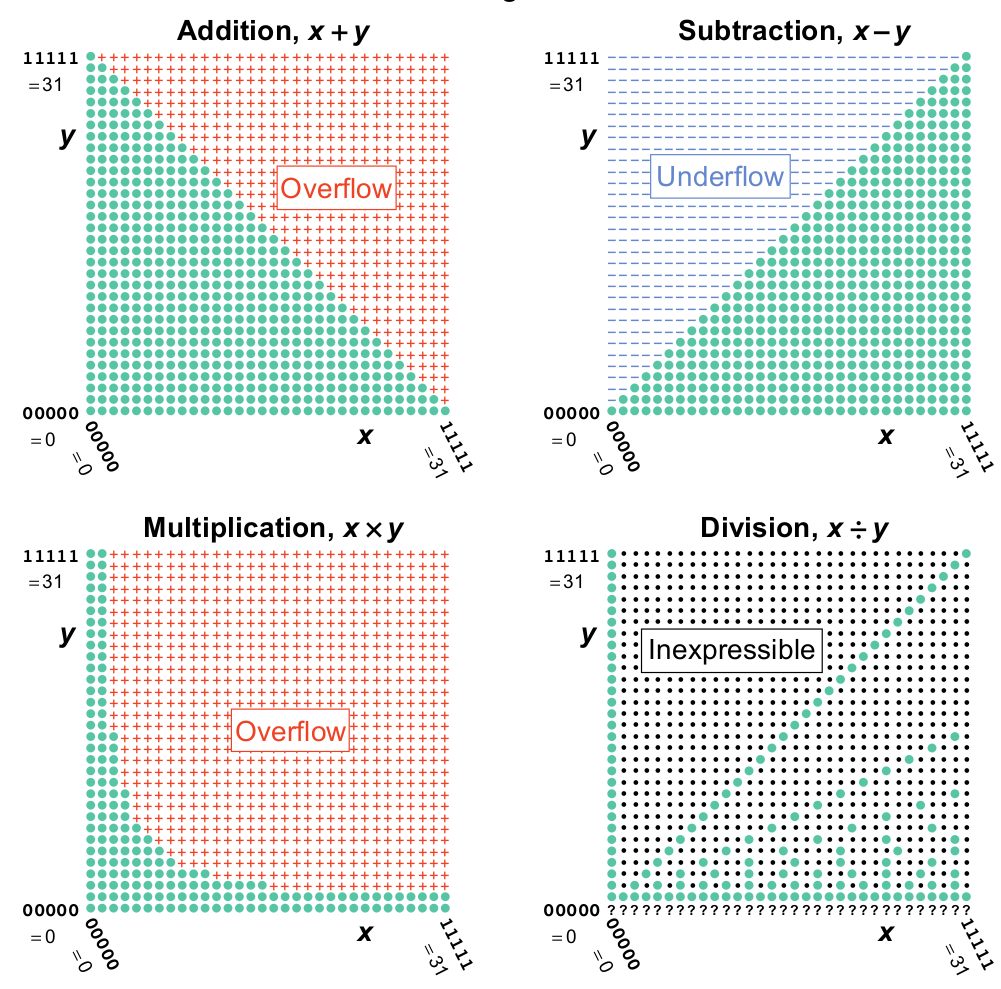
\includegraphics[height=9.7cm,width=0.7\textwidth]{book}
    \caption{A graphical view of bit strings: Value and closure plots from THE END of ERROR Unum Computing book at page number 9}
    \label{book}
\end{figure}
\newpage
\subsection{Intended Audience and Reading Suggestions}
This report is intended for readers who have studied Computer Science or similar, or are simply interested in the field of IT. Readers are assumed to have basic programming knowledge and some familiarity with web development technologies.

\subsection{Purpose}
The purpose of this report is divided into two purposes:\\

The first purpose is to describe the UI to CPBA application for instructors and Computer Science students at the Department of Computer Science - University of Copenhagen, so they can easily interact with the application.\\

The second purpose is to explain the requirement specifications for CPBA application and to explain the steps of implementing this project to help the developers to further develop the application.

\subsection{Project Scope}
CPBA will allow students to learn about the behaviour of basic arithmetic operations in floating point arithmetic with different Bit-Width through interaction with UI. The CPBA will also allow the instructors and creative students to modify the variables in arithmetic operations to monitor behaviour of floating point.%\\
%The objective of the CPBA application is to create a visualization tool that illustrates the behaviour of basic arithmetic operations (e.g., Addition, Subtraction, Multiplication, Division) in floating point arithmetic with different bit-width (e.g. Half, Single, Double, Quadruple).\\

\section{Overall Description}\label{Overall Description}
Floating point is the formulaic representation of a real number that includes all the rational numbers, such as the integer (negative, postive), the fraction, and all the irrational numbers, such as square root or  transcendental numbers.\\

Floating-point arithmetic is a subject that is considered exciting for many people, because the result of Floating-point arithmetic operations depends on the bit-width of the Floating-point. This is rather surprising because the floating-point bit-width can be the reason why it gives a different result. Almost every programming language has a floating-point datatype. Therefore, the use of two or more programming languages (for some common arithmetic calculations to develop a project) depend on Floating-point arithmetic operations that can give surprising results. The reason for that is, these programming languages have different bit-width and Floating-point datatypes, and also, bit-width differs from one computer to another computer. c.\ref{1}\\

The most popular code for representing real numbers is called the IEEE Floating-Point Standard c.\ref{2}, it has three basic components: the sign, the exponent, and the mantissa. The mantissa is composed of the fraction and an implicit leading digit. The exponent base (2) is implicit and does not need to be stored.\\

\subsection{Product Perspective}
A simple way to illustrate the behaviour of basic arithmetic operations is to physically sit in front of a computer or with paper and write down the numbers and finish the calculation process. There are tools available, commercial or open source, that support arithmetic operations to digits or binary numbers. Many operating systems and applications come with calculator support with basic arithmetic operations. However, all these tools usually require a person physically sitting in front of a computer writing down the numbers one by one.\\
\\Thus, there is a need for a web based application such as a visualization tool for illustrating the behaviour of basic arithmetic operations.

\section{Analysis}
In this section I will give an analysis of the problem described above. The analysis will focus on narrowing in special areas of the problem domain that will be central to designing \ref{Design} and implementing \ref{Implementation} a working prototype.
\subsection{Fixed Bit String}
There is obvious weakness when designing CPBA application, this weakness is the ability of the programming languages to represent integer number. The humans capable of representing unlimited integer number, but the situation is different to programming languages.  As I mentioned in section "Overall description" \ref{Overall Description}, Almost every programming language has a floating-point datatype. Therefore, table \ref{mathNo} shown the maximum integer that can be represent at some web development technologies.\\
\begin{table}[h]
\label{mathNo}
\scriptsize 
\centering
\begin{tabular}{|l|c|c|c|}
\hline
\multirow{2}{*}{\diagbox[width=8em]{Bit-width}{PL}}
                   & \multirow{2}{*}{JavaScript} & \multirow{2}{*}{Python}                 &\multirow{2}{*} {GO} \\ 
                   &                             &                                         &   \\ \hline
$2^{16}$      & 65536                       & 65536                                   &  65536\\ \hline%Half ~\ ~\ ~\ ~\ ~\ 
$2^{32}$    & 4294967296                  & 4294967296                              &  4.294967296e+09 \\ \hline%Single~\ ~\ ~\ ~\ 
$2^{64}$    & 18446744073709552000        & 18446744073709551616                    &  1.8446744073709552e+19 \\ \hline%Double ~\ ~\ ~\ 
$2^{128}$ & 3.402823669209385e+38       & 340282366920938463463374607431768211456 &  3.402823669209385e+38  \\ \hline%Quadruple ~\ 
\end{tabular}
\caption{Representation of integer from some programming languages}
\end{table}\\
From the above table \ref{mathNo}, I can see maximum integer can be exactly represented is in bit-width single, but for double and quadruple the integer has been represented as rounding numbers or in scientific notation.

%integer which cannot be exactly represented

%is incapable
%There is obvious weakness when designing CPBA application, this weakness is the size of bit-width. The humans capable of representing unlimited size of bit-width to integer, because 

%by their arithmetic notation definition.\\

%Different mathematical notation for floating point precision is one of the obvious shortcomings for designing CPBA application, if we could not represent those different precision with their actual mathematical notation.

\subsection{Rectangle Size vs Bit Pixel}
The browser window is the rectangle that a web page fills on screen. It is basically the size of the browser window, without the toolbars and scrollbars \ref{4}. I will use this window to visualize and illustrate the behaviour of basic arithmetic of Floating-point. But is it possible for the CPBA application to illustrate the behaviour of this basic arithmetic operations in this window !?\\

I want to calculate arithmetic operations with integer numbers that have different bit-width. To do these calculations I need at least two variables. That is, if the variables X and Y have Half bit-width I have to represent the result of this arithmetic operations, which results in $65536^{2} = 4294967296$ elements. This huge number of elements can not be shown in the browser window while maintaining a clear vision for each element separately. So I need some way to allow me to achieve a clear vision for each element, and also allow the user to take advantage of this visualization tool for illustrating the behaviour of basic arithmetic operations.\\
\section{Design}\label{Design}
I decided that it should be web-based so the application is easily accessible for students. In other words, it should be accessed via the internet by using a standard web browser or students can access the project files from a physical source (e.g. flash memory). This way there is no need for distributing the program and all the required packages for it to run, which I would need if I had to make a program that was not web-based. By making the application web-based I ensure its accessibility for most, if not all users.
The solution will not target mobile/tablet users specifically.\\

Now that the project is a web-based application I need to use HTML and CSS - seeing that they are the two core technologies for building Web pages. However, to build the functionality of this project I can choose between many programming languages, but JavaScript is the only one that fits the CPBA requirements. This way the users can access the CPBA online, and offline if they get the project from a physical source.\\

I discussed some of the problems that I will be confronted with in the design and implementation of the project in the above section (Analysis). Therefore, in the below subsection I will present the problems mentioned above and explain my ideas for the design and implementation of the solution to the problems.
\subsection{Arithmetic operations \& Different bit-width}
The user needs a simple way to illustrate the behaviour of basic arithmetic operations with different bit-width. Therefore, the project should make it possible for users to select and choose between different arithmetic operations and different bit-width. For this reason, I've decided that the front-end design of CPBA should include  two  <select> elements which create a drop-down list, and thereby I collect user input from the selected option.
\subsection{Mathematical notation}
Since I have chosen javascript as the primary programming language to the functionality of this project, it will provide access for the user whether it be online or offline. But does Javascript represent bit-width such as the way in which it represent in mathematical notation? Unfortunately, The answer is No because the maximum integer represented in JavaScript is $2^{53}+1$. Otherwise the integer will be represented in scientific notation. That's why I decided to make CPBA is limited to bit-width Half and Single only.
\subsection{Elements}
Representing fixed bit string equal to the length of bit string at bit-width Half and Single would produce huge number of elements. Those numbers would need to be shown in the browser window, but to represent all those elements at once will not make it possible for users to see and illustrate the behaviour of basic arithmetic operations. Therefore, the CPBA application needs to summarize those elements to miniature form.\\
Those miniature forms differ from one bit-width to another bit-width in the number of stages. In other words, for example at the addition operation to two variables of bit-width Half, that have $2^{16}$ elements for variable X and $2^{16}$ for variable Y, so the sum of those two variables is $2^{32}$ elements.\\\\
I decided to show 256 elements of this result at each stage, where each element represents 4 edges from the real results as shown in figure \ref{edges}.\\
\begin{figure}[h]
    \centering
    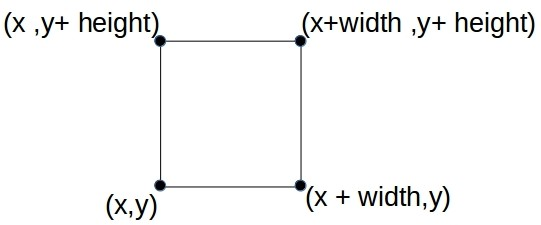
\includegraphics[width=0.5\textwidth]{edges}
    \caption{summarize form shows how each element represents in CPBA}
    \label{edges}
\end{figure}\\
The bit-width Half will have four stages. At the first stage width and height will be equal to 4095, at the second stage they will be equal to 255, at the third stage they will be equal to 15,  and at the fourth (last stage) they will be be equal to 0.\\\\
The bit-width Single will have eight stages. At the first stage width and height will be equal to 268435455, at the second stage they will be equal to 16777215, at the third stage they will be equal to 1048575, at the fourth stage they will be be equal to 65535, at the fifth stage they will be be equal to 4095, at the sixth stage they will be be equal to 255, at the seventh stage they will be be equal to 15, and at the eighth stage (the last one) they will be be equal to 0\\\\
The below examples is illustrative examples to prove the concept of the addition operation with bit-width Half at first stage form:\\\\
X = 4096, Y=53248\\
\scalebox{0.9}{
\begin{tabular}{lllll}
Leftmost bottom: &  4096  + 53248  &= 57344                  & ,57344  is less then $2^{16}$    & Correct\\
Rightmost bottom:& (4096 + 4095)  + 53248 &= 61439           & ,61439  is less then $2^{16}$    & Correct\\
Leftmost upper:  & 4096   + (53248 + 4095) &= 61439          & ,61439  is less then $2^{16}$    & Correct \\
Rightmost upper: & (4096  + 4095)  + (53248 + 4095) &= 65534 & ,65534  is less then $2^{16}$    & Correct\\
\end{tabular}
}\\\\
There are 4 correct and 0 Overflow, therefor i will show single Correct element represent this above range.\\\\
X = 4096, Y=57344\\
\scalebox{0.9}{
\begin{tabular}{lllll}
Leftmost bottom: &  4096  + 57344  & = 61440                  & ,61440  is less then $2^{16}$    & Correct\\
Rightmost bottom:& (4096 + 4095)  + 57344 & = 65535           & ,65535  is less then $2^{16}$    & Correct\\
Leftmost upper:  & 4096   + (57344 + 4095) & = 65535          & ,65535  is less then $2^{16}$    & Correct \\
Rightmost upper: & (4096  + 4095)  + (57344 + 4095) & = 69630 & ,69630  is more then $2^{16}$    & Overflow\\
\end{tabular}
}\\\\
There are 3 correct and 1 Overflow, therefor i will show single Mix element represent this above range.\\\\
%65536 65536
X = 4096, Y=61440\\
\scalebox{0.9}{
\begin{tabular}{lllll}
Leftmost bottom: &  4096  + 61440  & = 65536                  & ,65536  is more then $2^{16}$    & Overflow\\
Rightmost bottom:& (4096 + 4095)  + 61440 & = 69631           & ,69631  is more then $2^{16}$    & Overflow\\
Leftmost upper:  & 4096   + (61440 + 4095) & = 69631          & ,69631  is more then $2^{16}$    & Overflow \\
Rightmost upper: & (4096  + 4095)  + (61440 + 4095) & = 73726 & ,73726  is more then $2^{16}$    & Overflow\\
\end{tabular}
}\\\\
There are 0 correct and 4 Overflow, therefore, i will show single Overflow element representing this above range. 

\subsection{Forward, Back \& Reset}
Since there will be many stages, whether it be for bit-width Half or bit-width Single. Therefore, users need  to an mobility option, that can let the users move forward to next stage, back to previous stage or jump backward to first stage (Reset). \\

For achieving the mobility options to the user, I must provide a tool that allows the user to interact with presented data and the stages. This tools can be buttons, those buttons have to be available to user on UI.\\

To move forward to the next stage the user has to click on the element, thereafter, the clicked element will be the first element of the next stage, and so on until width and height are equal to zero. And, hereby the user has reached the final stage.\\\

To move back to previous stage the user clicks on the back button, that button will provide the option of going back to the previous stage until width and height are equal to value 4095 in bit-width Half or value 268435455 in bit-width Single.\\

To reset or to jump back to the first stage will be done by clicking on reset button, that button will assign width and height to 4095 in bit-width Half or 268435455 in bit-width Single.

\section{Implementation}\label{Implementation}
In this section I will explain the involved steps of the CPBA application's implementation. The Implementation steps are split into two parts (User Interface-UI and Back-end)
\subsection{UI}
For the implementation of the user interface I have chosen to use Bootstrap\footnote{Bootstrap, a front-end framework for web development \ref{http://getbootstrap.com/}}. Bootstrap is a front-end framework for web development, and helps me flesh out the user interface, ensuring that it looks the same no matter what browser the user is using to access the CPBA application.\\\\
In the UI I have implemented two select option elements, one to define the available options for bit-width, and the second one is to define the available options for arithmetic operations.\\
The selection option element for the different bit-width has the onchange attribute that assigns to getBit-Width() JavaScript function, that function is responsible for creating arrays of the different width and height values. The HTML code for select option is shown in the code snippet \ref{lst:Select option} at Appendix section \ref{app:A}.\\

I defined "Plot my requests" button element at the same div element for the select option to get the value of the selected option. This button has attribute onclick, which is to assign to JavaScript functions getRequest(); and showService();. getRequest() function will get the value of the selected option and I will explain this function clearly at the Back-end section. But showService() function is responsible for showing Back and Reset buttons, because those buttons are invisible until the user has clicked on Plot my requests button. I assigned the style display of those buttons to "none", thereby showService() will assign style display to "block" instead of none, thereby those buttons will be shown in UI.\\
The HTML code for "Plot my requests" button is shown in the code snippet \ref{lst:Plot my requests} at Appendix section \ref{app:A}, the HTML code for Back and Reset buttons is shown in the code snippet \ref{lst:select option button}, and the JavaScript code for showService() function is shown in the code snippet \ref{lst:showService} at Appendix section \ref{app:A}.\\

Figure\ref{UI} show the last version of UI that I created for the CPBA application.
\begin{figure}[h]
    \centering
    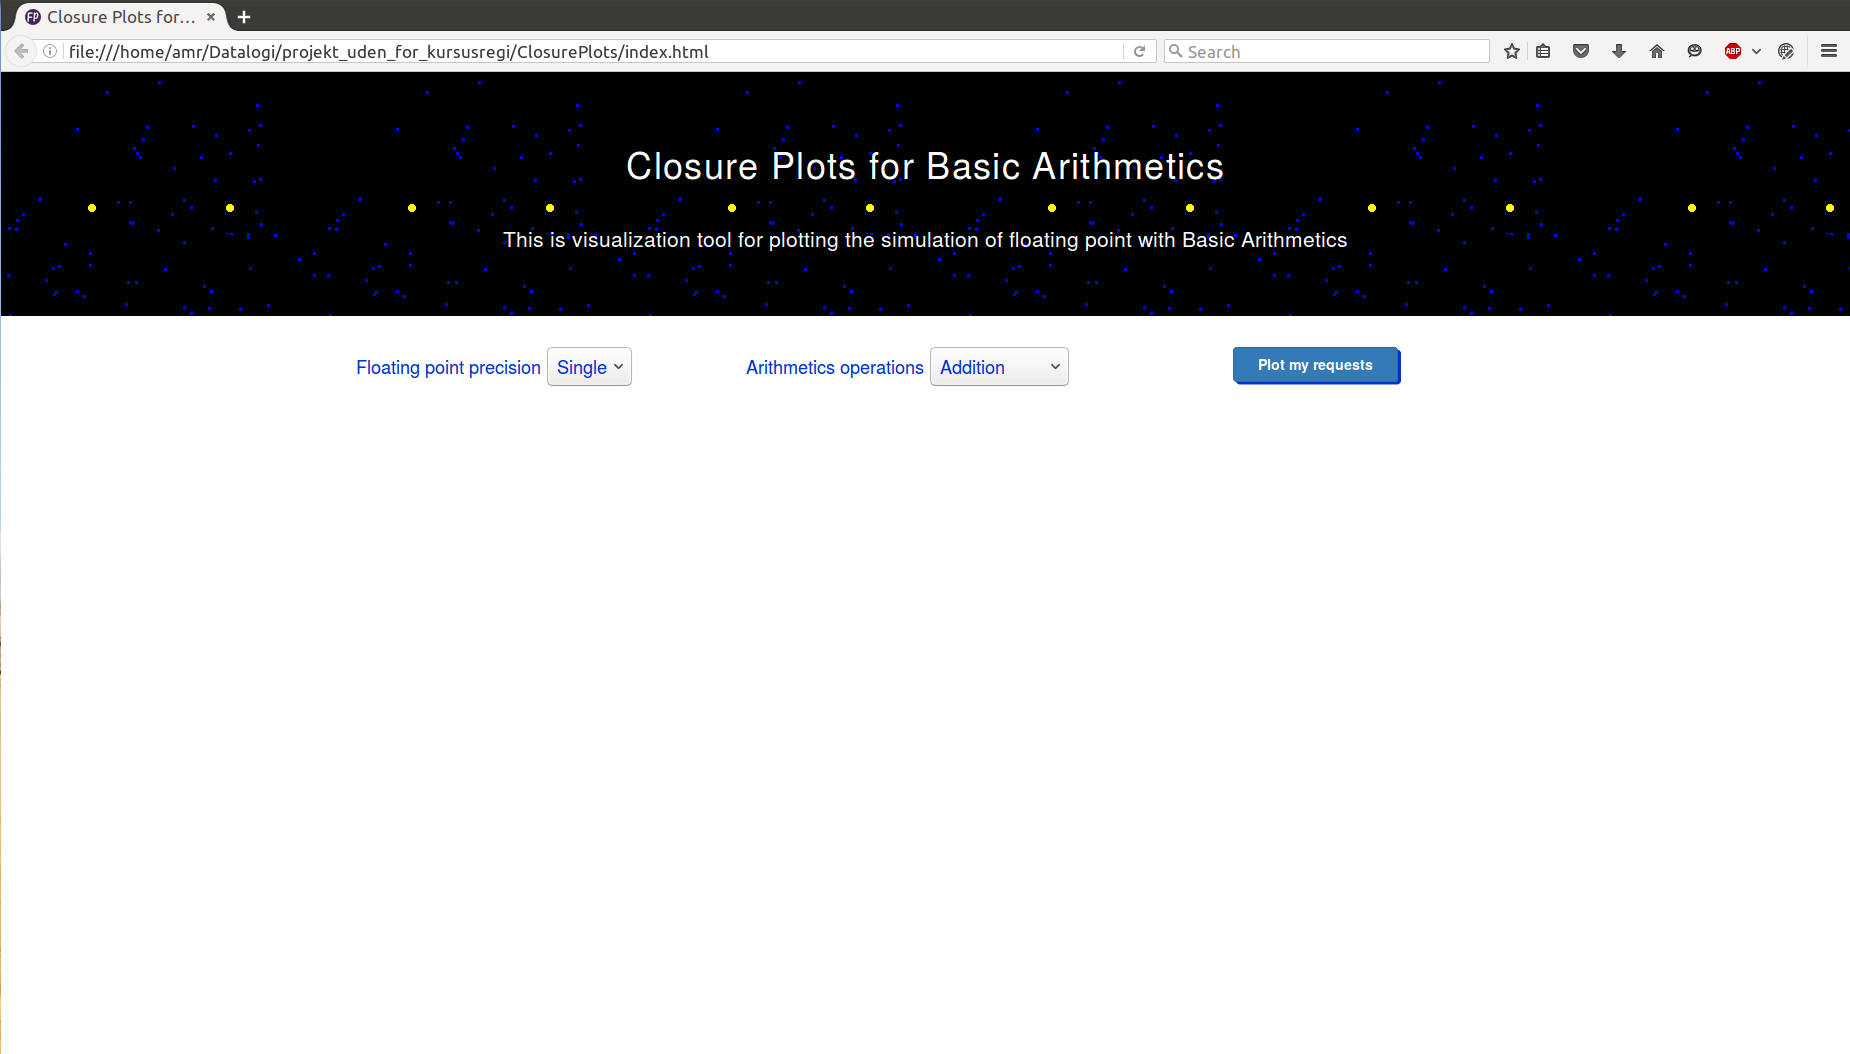
\includegraphics[width=1\textwidth]{layout}
    \caption{CPBA application UI}
    \label{UI}
\end{figure}\\
\subsection{Back-end}
In the design section I described that I would use javascript to implement the back-end functionality. The back-end consists of many functions, I will review these functions based on their order of the implementation to the CPBA application. But, before the review of these functions, i would like to show the outline of implementation the arithmetic operations.\\
\\The arithmetic operations at this project will have same algorithms for implementation except checking the behaviour of variables (correct, overflow, underflow, inexpressible, infinity). The below steps describing the algorithm for implementing those arithmetic operations.
\begin{enumerate}
\item Get the requested bit-width. For two reasons:
  \begin{enumerate}
    \item Define array of the values for width and height.
    \item Assign the requested bit-width to variable. 
  \end{enumerate}
\item Get the requested arithmetic operation. So I can call the appropriate function.
\item Check the x and y values.
\item Summarize the edges for elements at each stage based on height and width value.
\item Check the behaviour of elements at the edges.
\item Represent the binary value of the summarize elements.
\item Visualize the data
\end{enumerate}

\subsubsection{getBit-Width() function.}
The first call occurs when the body of the webpage has been loaded. The second call occurs when the user changes the select option to bit-width. getbit-width receives the value of bit-width select option, which is 16 for Half bit-width or 32 for single bit-width. The function starts by initializing the global precArr variable to empty array, and initializing the global mobile variable to 0. Thereafter, assigns variable temp the return value of base 2 to the exponent power of bit-width value ( 16 or 32).
Now the function is ready to create the width and height value to the selected bit-width, and that is done by a while loop as long as a specified condition ((temp/16) >= 1) is true. Inside the scope of while loop I divide the value of temp variable by 16, and then push the return value of temp -1 to precArr array. The while loop will create array of width and height values.\\

The return value for precArr variable when bit-width is half will be \textit{[4095, 255, 15, 0]}, and the return value for precArr when bit-width is Single will be \textit{[268435455, 16777215, 1048575, 65535, 4095, 255, 15, 0]}.\\
\\The JavaScript code for getBit-Width() function is shown in the code snippet\ref{lst:getBit-Width} at Appendix section \ref{app:A}.\\

\subsubsection{getRequest() function.} 
This function is called when the user has clicked on the "Plot my requests" button. The function starts with defining a variable "op" and assigning this variable to the value of select option "operations", which are addition, subtraction, multiplication, or division. Thereafter, it defines a switch statement and evaluates variable "op " value to match the value to a case clause, and executes function associated with that case.\\
The JavaScript code for getBit-Width() function is shown in the code snippet\ref{lst:getRequest} at Appendix section \ref{app:A}.\\

\subsubsection{function add()}
The add() function calculates the sum of two variables in arithmetic operation. Also, it shows the behaviour of this arithmetic operation ( Correct, overflow ). It will be executed when it's called by function getRequest().\\
The body of add() function starts with a variable prec definition, this variable will be assigned to the value of the bit-width selected option. Thereafter, a variable range is defined - this variable will be assigned to the return value of base 2 to the exponent power of prec value.
The height and width variables are assigned to the values of precArr[mobile], where precArr and mobile have been created from getBit-Width() function.
Thereafter, variable index 0 is intialized to 0, and variable row is initialized to an empty array. The variable index will be used to insert specified items to array row. The variables f1 and f2 are defined to assign the values of X and Y to them after their values have been converted to binary format.\\

The next variable is getPixel, this variable declares a function expression in the current scope of add() function. getPixel will summarize 4 edges of 256 elements at each stage based on height and width value. In the current scope of getPixel function I define variable check. This variable declares a function expression - the function checks the sum of items at each edge for the 4 edges of 256 elements: if the result of the edge is less than the value of range variable the correct variable is increased by 1,  otherwise the variable overflow is increased by 1.\\

The next step is to represent the result of the summarized data, and that is done by checking if the value of the correct variable is greater than 0 and the value of overflow variable is equal to 0, so the summarized data will be shown to user as it is correct data. Or, if the value of overflow variable is greater than 0 and the value of correct variable is equal to 0, so the summarized data will be shown to the user as it is overflow data. Other than that, the summarized data will be shown to the user as it is mixed data (correct and overflow).\\

At lines 40-42 of the snipped code, I defined variables xV and yV, those variables will be assigned to the value of variables xValue and yValue. The variables xValue and yValue have been defined as global and have been initialized to null value as shown in the snapped code \ref{lst:xyvalue-global} at Appendix section \ref{app:A}. Therefore, at the first stage xV and yV will be assigned to 0. However, if the user clicks on an item of the represented data, the values of this item will be assigned to xValue and yValue variables and thereby xV and yV will be assigned to xValue and yValue.\\

The getFormat variable is a declare function expression in the current scope of add() function. I defined getFormat function with one parameter, this parameter passes from prec variable to the decBin function \ref{lst:decBin}, and the return value of decBin is assigned to the variables f1 and f2, where those variables will represent the binary value of x and y items of the shown data.\\

At lines 47-57 I define two for loops. The first loop represents the x-axis items, and the second loop represents the y-axis items.
The first loop has 16 iterations, and in the beginning of the loop I started by assigning variable x to the value of variable xV. And, at each iteration the x value is updated to its value plus width value. Thereafter, I call getFormat function with x value to get the binary value of x, so i can show it to the user. The next variable is dicX, this variable is an object with two properties key and value, and it is defined like that to fit Google Chart API to represent the items. The value for v key is x value, and the value of f key is the binary value of f1 to f2.\\
The second loop is defined in the body of the first loop, it also has 16 iterations. I started the same way as the previous loop, but this time it assigns variable y to the value of variable yV, and at each iteration the y value updates to its value plus height value. Thereafter, I call getFormat function with y value to get the binary value of y so i can show it to the user. I defined variable dicY as an object with two properties key and value. The value for v key is y value, and the value of f key is the binary value of f1 to f2. Now I can call getPixel to summarize the 4 edges, and that is done by passing variables x, y , height, width, dicX, and dicY to the getPixel function.\\
This two loop produces 256 elements, those elements were inserted at row array at getPixel function, therefore, at line 58 I called drawChart() function to visualize the data for the user. At the next subsection I will review and explain drawChart() \ref{lst:drawChart} function and how it works.\\

\subsubsection{function drawChart(arg1, arg2) }
This function plots the received data from add, sub, mult, and divi functions. The function takes two arguments, the first argument is the desired display data, and the second argument is an array of legends to describe the shown data (e.g. correct, Overflow, Underflow, Inexpressible, infinity, and mix). While the function will get different lengths in the second argument, I need to check the length of the second argument to pass the right legend to the shown data. If the length of arg2 is equal to three the received data is from divi() function, and thereby the legend will refer to 4 different data ( Correct, Inexpressible, Infinity, and Mix). Otherwise the legend will refer to 3 different data (Correct, (Overflow or Underflow), and Mix). Thereafter, adds new rows to the data table - the rows are arrays that have been passed to the drawChart parameter. Line 21 is to configure the options of the chart, where I defined the char title, width and height. At line 28 variable chart is an object of class google.charts.Scatter,  where "chart\_div1" div is used to contain the chart drawn.\\

In the scope of drawChart function I have defined selectHandler() function, this function will allow users to interact with the shown data by clicking on the items, and thereby I get the x and y values of the clicked item. Those values are assigned to the global variables xValue and yValue. At line 51 I have defined variable valid, and it's assigned to the return value of checkIndex() function. This function checks if the mobile variable has not run out of range to precArr length as shown in the snapped code \ref{lst:checkIndex} at Appendix section \ref{app:A}. If the return value of checkIndex is true then increase the value of variable clickIndex by 1, and call getRequest() function.

\subsubsection{function sub()}
The sub() function \ref{lst:sub} calculates the subtraction of two variables in arithmetic operation. And, the function is to show the behaviour of this arithmetic operation ( Correct, Underflow ). The function will be executed when it's called from function getRequest() \ref{lst:getRequest}. The sub() function has the same definition like the add() function \ref{lst:add} except the logic for check() function.\\
\\At the scope of sub() function, the check() function checks if the result of left expression subtract the right-side expression for the items at the four edges of 256 elements. If the result is greater than zero and the result is less than or equal to range variable the correct variable increased by 1. Otherwise the variable underflow is increased by 1 as shown in the snapped code \ref{lst:sub} lines 20-22 at Appendix section \ref{app:A}.\\

\subsubsection{function mult()}
The mult() function \ref{lst:mult} calculates the multiplication of two variables in arithmetic operation. And, the function is to show the behaviour of this arithmetic operation ( Correct or Overflow ). The function will be executed when it's called from function getRequest() \ref{lst:getRequest}. The mult() function has the same definition like the add() \ref{lst:add}, and sub() \ref{lst:sub} functions except the logic for check() function.\\
\\At the scope of mult() function, the check() function checks if the result of left-side expression multiplication the right-side expression for the items at the four edges of 256 elements. If the result is less than range variable the correct variable increased by 1. Otherwise the variable overflow is increased by 1 as shown in the snapped code \ref{lst:mult} lines 20-22 at Appendix section \ref{app:A}.\\

\subsubsection{function divi()}
The divi() function \ref{lst:divi} calculates the division of two variables in arithmetic operation. And, the function is to show the behaviour of this arithmetic operation (Correct, Inexpressible "Numbers do not divide evently", Infinity "Numbers divide by zero" ). The function will be executed when it's called from function getRequest() \ref{lst:getRequest}. The divi() function has the same definition like the add() \ref{lst:add}, sub() \ref{lst:sub}, and mult() \ref{lst:mult} functions except the logic for check() function.\\
\\At the scope of divi() function, the check() function checks if the result of left-side expression divide by the right-side expression modulus 1 is equal to zero for the items at the four edges of 256 elements. If the condition is true the correct variable increased by 1, else if left-side  expression divide by right-side expression is Not a Number (e.g. 0/0) or left-side expression divide by right-side expression is not finite (e.g. 1/0, 2/0 , .., n/0), then the fini variable increased by 1. Otherwise the variable Inexpressible increased by 1 as shown in the snapped code \ref{lst:mult} lines 21-26 at Appendix section \ref{app:A}.\\

\subsubsection{function reset()}
The purpose of reset() \ref{lst:reset} function is to reset chart and go back to first stage to show the previous data at this stage. The function reset() begins by reassign variable mobile value to zero, thereafter reassign global variables xValue and yValue values to null, and at last reassign variable clickIndex value to zero, then it call getRequest() function. The onclick event occurs when the user clicks on reset button at UI, then 
the reset() function will be execute.\\
The reset() function will be execute when onclick event occurs while the user clicks on reset button at UI. The code for reset function shown in the snapped code \ref{lst:reset} at the Appendix section \ref{app:A}.

\subsubsection{function getBack()}
The purpose of getBack() \ref{lst:getBack} function is to allow user to move back to the previous stage, if and only if the user has moved forward. The implementation of this function is based on stack (Last In First Out), where selectHandler() \ref{lst:drawChart} function allow users to interact with the shown data and move forward by clicking on the items, so I save the clicked value of x to array clickedX and save the clicked value of y to clickedY. But, when user clicks on getBack button at UI (onclick event occurs), than getBack() function will be executed and global variable xValue will be assign to last item at clickedX array, and yValue will be assign to last item at clickedY array. To keep track the last elements of clickedX and clickedY, I had defined variable clickIndex, that point to the last index of clickedX and clickedY arrays at selectHandler() function. The clickIndex variable value is increasing by 1 when user clicks on data elements, and it is decreasing by 1 when user clicks on getBack button.

\section{Testing}
In this section I will give some screenshots of the tests that I have done to the CPBA application and explain these screenshots.\\
At Figure\ref{offline} I have tested the possibility that the users can access the CPBA at offline mode. And, yes the users can access the CPBA application, if they get the application from a physical source, because the stylesheet of bootstrap will be delivered with the application.\\\\
At Figures\ref{half-add} \ref{half-sub} \ref{half-mult} \ref{half-div} I have tested if the users can select bit-width half to (Addition, Subtraction, Multiplication, Division) operations. And, as we can see at those figures, when the user select half bit-width and the arithmetic operations, and thereafter the user can click on "Plot my requests" button and the data will be shown in the center of browser window. As well as, if users chose single bit-width as shown at Figures \ref{single-add} \ref{single-sub} \ref{single-mult} \ref{single-div}.\\\\
I have also tested, if the user can interact with the chart, and clicked on some elements. As we can see at figure \ref{first-stage}, this figure refers to the first stage for Half bit-width and arithmatic operation addition. The chart show the first element at x-axis is 0 and the last element is little bit more than 64k (k refers to  thousand). I have hovered over the last element to x-axis, which is also the first element to y-axis, we can see the Pop-up windows show x value is range of 1111000000000000 - 1111111111111111, and y value is range of 0000000000000000 - 0000111111111111. And, By click on this element we moved to the next stage as shown in figure \ref{second-stage}. At the second stage by hover over the last element to x-axis we can see the Pop-up windows show the value of x is range of 1111111100000000 - 1111111111111111, and y value is range of 0000000000000000 - 0000000011111111. Again, By click on this element we moved to the next stage as shown in figure \ref{third-stage}.At the third stage by hover over the last element to x-axis we can see the Pop-up windows show the value of x is range of 1111111111110000 - 1111111111111111, and y value is range of 0000000000000000 - 0000000000001111. Lastly, By click on this element we moved to the next stage as shown in figure \ref{last-stage}.At the this stage we are at last stage by hover over the last element to x-axis we can see the Pop-up windows show the value of x is range of 1111111111111111 - 1111111111111111, and y value is range of 0000000000000000 - 0000000000000000.\\
I have tested the reset button and it do the reset functionality as how it should be, where the chart has been moved to its first stage. I have also tested the getBack button, but it has bug.\\

%\section{Future Development}
%\section{Work progress}
\section{Conclusion}
In this report I have presented an idea for an application that can illustrate the behaviour of basic arithmetic operations in Floating-Point arithmetic with different bit-width, so the students of the Department of Computer Science - University of Copenhagen can learn and interact with this application.\\

The primary goal to this project was to reproduce the graphical view from John L. Gustafson book (THE END of ERROR Unum Computing) that illustrating the behaviour of bit-width representation for basic arithmetic operations.\\

I decided to use CSS, HTML5, and JavaScript as the technologies that were needed to develop the application, and for the data visualization, i have used Google Chart.\\

I had implemented this application so that it can to be easily accessed via the internet by using a standard web browser or students can access the application files from a physical source.\\

I had implemented a visualization tool for illustrating the behaviour of basic arithmetic operations (Addition, Subtraction, Multiplication, Division) to integer with a fixed-size of bit string, which refer to the same size of bit-width (Half $2^{16}$ , Single $2^{32}$), and also i had explained why i couldn't implemented for  bit-width( Double $2^{64}$ , Quadruple $2^{128}$)\\

For the future development, even I didn't explained how it's possible to extend this project with some other arithmetic operation or illustrating the behaviour of decimal numbers, rational numbers, and all the irrational numbers in Floating-Point, but i strongly beleive that the implementation of this project might be useful for  future development to fit some other arithmetic operation and fit some other real numbers.

\newpage
\section*{References}
\begin{enumerate}[label={[\arabic*]}]
\item \label{1}
\scalebox{0.9}{
\begin{tabular}{lll}
  Author  &:& Goldberg, David\\
  Title   &:& What Every Computer Scientist Should Know About Floating-point Arithmetic\\
  Journal &:& ACM Comput. Surv.\\
  date    &:& March 1991 
\end{tabular}
}
\item \label{2}
\scalebox{0.9}{
\begin{tabular}{lll}
  Author  &:& American National Standards Institute and Institute of Electrical and Electronice Engineers\\
  Title   &:& IEEE Standard for Binary Floating-Point Arithmetic\\
  Date    &:& 21.March 1985\\
  url     &:& http://www.wellposed.com/standards-documents-cache/IEEE754-1985.pdf
\end{tabular}
}
\item \label{3}
\scalebox{0.9}{
\begin{tabular}{lll}
  Author  &:& John L. Gustafson\\
  Title   &:& THE END of ERROR Unum Computing\\
  V-Date  &:& 12.November 2014\\ 
  ISBN    &:& International Standard Book Number-13: 978-1-4822-3987-4 (eBook - PDF)
\end{tabular}
}
\item \label{4}
\scalebox{0.9}{
\begin{tabular}{lll}
  Author  &:& James Royal-Lawson\\
  Title   &:& What is my viewport size and pixel density?\\
  Date    &:& 2013-05-05\\ 
  url     &:& http://beantin.se/what-is-my-viewport-size-pixel-density
\end{tabular}
}
\end{enumerate}

%%\addcontentsline{toc}{section}{References}
%\bibliographystyle{ieeer}
%%\bibliographystyle{unsrtnat}
%%\bibliography{ref}

\section*{Footnotes}
\begin{itemize}
\item \url{http://steve.hollasch.net/cgindex/coding/ieeefloat.html}
\item \url{https://developers.google.com/chart/}
\item \url{http://getbootstrap.com/}
\end{itemize}

\newpage
\section{Appendix} \label{app:A} %Appendices
\begin{lstlisting}[label={lst:Select option}, language=HTML, caption={Select option for bit-width and arithmetic operations},]
  <div class="row">
      <div class="col-md-4">
        <font>Floating point bit-width</font>
        <select id="bit-width" onchange="getBit-Width();">      
          <option value="16">Half    </option>
          <option value="32">Single  </option>
        </select>
      </div>

      <div class="col-md-4">
        <font>Arithmetics operations</font>
        <select id="operations" > 
          <option value="addition">Addition</option>
          <option value="subtraction">Subtraction</option>
          <option value="multiplication">Multiplication</option>
          <option value="division">Division</option>
        </select>
      </div>
\end{lstlisting}


\begin{lstlisting}[label={lst:Plot my requests}, language=HTML, caption={Plot my requests button to get the value of the select option},]
        <button type="button" class="btn btn-primary" onclick="getRequest();showService();" 
          style="margin-top:1px;">
          <strong color="">Plot my requests</strong>
        </button>
  </div>      
\end{lstlisting}

\begin{lstlisting}[label={lst:select option button}, language=html, caption={Back and Reset buttons},]
    <div class="row" id="service" style="display:none;">
      <div class="col-md-2 col-md-offset-10">
        <div class="col-md-1" style="margin-right:10px;">
        <!--getBack()-->
          <button data-toggle="tooltip" data-placement="top" title="Back" type="button" 
            class="btn btn-link btn-circle" onclick="getBack();"><!--getBack-->
            <img style="width: 43px; height: 43px;margin:-11px 2px 0px -6px;" 
              src="img/playback.ico">
          </button>
        </div>

        <div class="col-md-1">
          <button data-toggle="tooltip" data-placement="top" title="Reset" type="button" 
            class="btn btn-link btn-circle" onclick="reset();">
            <img style="width: 43px; height: 43px;margin:-12px 2px 0px -7px;" src="img/reset.ico">
          </button>
        </div>
      </div>
    </div>
\end{lstlisting}

\begin{lstlisting}[label={lst:showService}, language=Javascript, caption={showService function will change style of buttons to block},]
      function showService() {
        document.getElementById("service").style.display = "block";
      }
\end{lstlisting}

\begin{lstlisting}[label={lst:getBit-Width}, language=Javascript, caption={getBit-Width function},]
/* getBit-wWidth Function is to create array of the different dimensional to chart.
 * The function has to reset mobile variable to zero, which will point to the start of precArr.
 * The function will be execute onload of the body element and when a user changes the selected 
 * option of a <select> element.
 */
var mobile = 0;
var precArr = [];

function getBit-Width(){
  precArr = [];
  mobile  = 0;
  var temp= Math.pow(2, document.getElementById("bit-width").value);

  while((temp / 16) >= 1){
    temp /= 16;
    precArr.push(temp-1); 
  }
}
\end{lstlisting}

\begin{lstlisting}[label={lst:getRequest}, language=Javascript, caption={getRequest function},]
/*  getRequest function is to create object of the selected options
 *  and call the appropriate function depending on user request.
 */
function getRequest(){
  var op = document.getElementById("operations").value;
  switch(op){
    case "addition":
      add();
      break;
    case "subtraction":
      sub();
      break;
    case "multiplication":
      mult();
      break;
    case "division":
      divi();
      break;
    default:
      alert('Something went wrong!\n'
        + 'Please contact the publisher and let the author know about the bug.\n'
        + 'amr11682@hotmail.com');
      break;
  }
}
\end{lstlisting}

\begin{lstlisting}[label={lst:add}, language=Javascript, caption={add function},]
// function to create the simulation of Arithmetics operation ( addition )
function add(){
  var prec  = parseInt(document.getElementById("bit-width").value);

  var range = Math.pow(2, prec);

  var height= precArr[mobile];
  var width = precArr[mobile];

  var index = 0;
  var rows  = [];

  var f1; // X-axis data format 
  var f2; // Y-axis data format

  var getPixel = function(x, y, height, width, dictX, dictY) {
    var correct = 0;
    var overflow = 0;
    
    var check = function(x,y) {
      if (x + y < range) { correct += 1; } else { overflow += 1; }  
    }
    check(x, y);
    check(x, y + height);
    check(x + width, y);
    check(x + width, y + height);
    if (correct > 0 && overflow == 0) {
        // Correct data
      rows[index] = [dictX, dictY, null, null];

    } else if(overflow > 0 && correct == 0) {
      // Overflow data
      rows[index] = [dictX, null, dictY, null];

    } else {
      // Mix data
      rows[index] = [dictX, null, null, dictY];
    }
  }
  var xV;
  var yV; 
  if(xValue == null && yValue == null){xV=0; yV=0;}else{xV = xValue; yV = yValue;}
  if(clickIndex > 0){clickedX.push(xV);clickedY.push(yV);}
  
  var getFormat = function(param){f1 = decBin(param, prec); f2 = decBin(param+height, prec);}
  //var x = 0
  for(var x = xV, i = 0; i < 16; i++, x += width+1){
    getFormat(x);
    var dictX = {v:x, f:'X: '+f1+' to '+f2};
    //var y = 0
    for(var y = yV, j = 0; j < 16; j++, y += height+1){
      getFormat(y);
      var dictY = {v:y, f:'Y: '+f1+' to '+f2};
      getPixel(x, y, height, width, dictX, dictY);
      index += 1;
    }
  }
  drawChart(rows, ['Overflow', 'Mix']);
}
\end{lstlisting}

\begin{lstlisting}[label={lst:xyvalue-global}, language=Javascript, caption={Global variables},]
// Declare global variable, which will get their value from drawChart function, 
// only if the user has interacted with chart ( click on (x,y) ). 
var xValue = null;
var yValue = null;

var clickedX = [];
var clickedY = [];
var clickIndex = 0;
\end{lstlisting}

\begin{lstlisting}[label={lst:decBin}, language=Javascript, caption={Convert (Decimal to Binary) with specify length of the output},]
/*  decBin function is to convert (Decimal to Binary) with specify length of the output.
 *  The function take 2 arguments ( dec, length)
 *  dec   : is the decimal number, which need to be convert to binary
 *  length: is the desirable bit-width. 
 *  The function convert positive decimal as well as negative decimal 
 */
function decBin(dec,length){
  var out = "";
  while(length--)
    out += (dec >> length ) & 1;
  return out;
}
\end{lstlisting}

\begin{lstlisting}[label={lst:drawChart}, language=Javascript, caption={drawChart function will visualize the passed data to user.},]
function drawChart(arg1, arg2) {
  // Define the chart to be drawn. 
  var data = new google.visualization.DataTable();
  data.addColumn('number', '');
  data.addColumn('number', 'correct');
  if (arg2.length == 3){
    // numbers do not divide evenly  (Inexpressible) 
    data.addColumn('number', arg2[0]);
    // divide by zero
    data.addColumn('number', arg2[1]);
    // Mixed
    data.addColumn('number', arg2[2]);
  } else{
    // Overflow or Underflow
    data.addColumn('number', arg2[0]);
    // Mixed
    data.addColumn('number', arg2[1]);
  }
   
    data.addRows(arg1);
    var options = {
      chart: {
        title: ' Plotting the simulation of floating point with Basic Arithmetics'
      },
      width: 1150,
      height: 500,
    };
    var chart = new google.charts.Scatter(document.getElementById('chart_div1'));

    chart.draw(data, google.charts.Scatter.convertOptions(options));
 

  // Listen for the 'select' event, and call my function selectHandler() when
  // the user selects something on the chart.

    google.visualization.events.addListener(chart, 'select', selectHandler);

    // This function to get the index of the selected element of chart.
  function selectHandler() {

    mobile += 1;

    var selectedItemRow = chart.getSelection()[0].row;
    var selectedItemCol = chart.getSelection()[0].column;

    if (selectedItemRow != null){

      xValue = data.getValue(selectedItemRow, 0);
      yValue = data.getValue(selectedItemRow, selectedItemCol);

      var valid  = checkIndex();

      if(valid){
        clickIndex += 1;
        getRequest();//xValue, yValue);
      }
    }
  };
}
\end{lstlisting}

\begin{lstlisting}[label={lst:checkIndex}, language=Javascript, caption={check if the mobile variable has not run out of range to precArr length.},]
/* checkIndex function is to check if the mobile variable 
 * has not run out of range to precArr length. 
 */
function checkIndex(){
  if(mobile < precArr.length){return true;}else{return false;}
}
\end{lstlisting}

\begin{lstlisting}[label={lst:sub}, language=Javascript, caption={sub function},]
// function to create the simulation of Arithmetics operation ( subtraction )
function sub(){//xValue, yValue){
  var prec  = parseInt(document.getElementById("bit-width").value);
  // range to iteration (loop)
  var range = Math.pow(2, prec);

  var height= precArr[mobile];
  var width = precArr[mobile];

  var index = 0;
  var rows  = [];

  var f1; // axis data format 
  var f2; // axis data format

  var getPixel = function(x, y, height, width, dictX, dictY) {
    var correct = 0;
    var underflow = 0;

    var check = function(x,y) {
      if ((x - y) >=0 && (x - y) < range) { correct += 1; } else { underflow += 1; }  
    }
    check(x, y);
    check(x, y + height);
    check(x + width, y);
      check(x + width, y + height);
        console.log(x,y,correct, underflow, dictX, dictY, index);
      if (correct > 0 && underflow == 0) {
        // Correct data
      rows[index] = [dictX, dictY, null, null];

    } else if(underflow > 0 && correct == 0) {
      // Overflow data
      rows[index] = [dictX, null, dictY, null];

    } else {
      // Mix data
      rows[index] = [dictX, null, null, dictY];
    }
  }
  var xV;
  var yV; 
  if(xValue == null && yValue == null){xV=0; yV=0;}else{xV = xValue; yV = yValue;}
  if(clickIndex > 0){clickedX.push(xV);clickedY.push(yV);}
  
  var getFormat = function(param){f1 = decBin(param, prec); f2 = decBin(param+height, prec);}
  //var x = 0
  for(var x = xV, i = 0; i < 16; i++, x += width+1){
    getFormat(x);
    var dictX = {v:x, f:'X: '+f1+' - '+f2};
    //var y = 0
    for(var y = yV, j = 0; j < 16; j++, y += height+1){
      getFormat(y);
      var dictY = {v:y, f:'Y: '+f1+' - '+f2};
      getPixel(x, y, height, width, dictX, dictY);
      index += 1;
    }
  }
  drawChart(rows, ['Underflow', 'Mix']);
}
\end{lstlisting}

\begin{lstlisting}[label={lst:mult}, language=Javascript, caption={mult function},]
// function to create the simulation of Arithmetics operation ( multiplication )
function mult(){//xValue, yValue){
  var prec  = parseInt(document.getElementById("bit-width").value);
  // range to iteration (loop)
  var range = Math.pow(2, prec);

  var height= precArr[mobile];
  var width = precArr[mobile];

  var index = 0;
  var rows  = [];

  var f1; // axis data format 
  var f2; // axis data format

  var getPixel = function(x, y, height, width, dictX, dictY) {
    var correct = 0;
    var overflow = 0;

    var check = function(x,y) {
      if (x * y < range) { correct += 1; } else { overflow += 1; }  
    }
    check(x, y);
    check(x, y + height);
    check(x + width, y);
    check(x + width, y + height);
    if (correct > 0 && overflow == 0) {
        // Correct data
      rows[index] = [dictX, dictY, null, null];

    } else if(overflow > 0 && correct == 0) {
      // Overflow data
      rows[index] = [dictX, null, dictY, null];

    } else {
      // Mix data
      rows[index] = [dictX, null, null, dictY];
    }
  }
  var xV;
  var yV; 
  if(xValue == null && yValue == null){xV=0; yV=0;}else{xV = xValue; yV = yValue;}
  if(clickIndex > 0){clickedX.push(xV);clickedY.push(yV);}
  
  var getFormat = function(param){f1 = decBin(param, prec); f2 = decBin(param+height, prec);}
  
  for(var x = xV, i = 0; i < 16; i++, x += width+1){
    getFormat(x);
    var dictX = {v:x, f:'X: '+f1+' to '+f2};
    //var y = 0
    for(var y = yV, j = 0; j < 16; j++, y += height+1){
      getFormat(y);
      var dictY = {v:y, f:'Y: '+f1+' to '+f2};
      getPixel(x, y, height, width, dictX, dictY);
      index += 1;
    }
  }
  drawChart(rows, ['Overflow', 'Mix']);
}

\end{lstlisting}

\begin{lstlisting}[label={lst:divi}, language=Javascript, caption={divi function},]
// function to create the simulation of Arithmetics operation ( division )
function divi(){//xValue, yValue){
  var prec  = parseInt(document.getElementById("bit-width").value);
  // range to iteration (loop)
  var range = Math.pow(2, prec);

  var height= precArr[mobile];
  var width = precArr[mobile];

  var index = 0;
  var rows  = [];

  var f1; // axis data format 
  var f2; // axis data format

  var getPixel = function(x, y, height, width, dictX, dictY) {
    var correct = 0;
    var infi    = 0;
    var Inexpressible = 0;

    var check = function(x,y) {
      if ((x/y) % 1 == 0) { correct += 1; }
      // Check if the result if NAN (e.g. 0/0) or the result is Infinity (e.g. 1/0, 2/0, ...)
      else if(isNaN(x/y) || !(isFinite(x/y))) { infi += 1;}
      else{ Inexpressible += 1; } 
    }
    check(x, y);
    check(x, y + height);
    check(x + width, y);
    check(x + width, y + height);
    if (correct > 0 && Inexpressible == 0 && infi == 0) {
        // Correct data: does (1/3) which is 0.33.. mod 1  equal to zero
      rows[index] = [dictX, dictY, null, null, null];

    } else if(Inexpressible > 0 && correct == 0 && infi == 0) {
      // Inexpressible data
      rows[index] = [dictX, null, dictY, null, null];

    }else if(infi > 0 && correct == 0 && Inexpressible == 0) {
      // check if is NAN eg. 0/0  or is Infinity(not finite)  eg. 1/0 , 1000/0
      rows[index] = [dictX, null, null, dictY, null];

    } else {
      // Mix data
      rows[index] = [dictX, null, null, null, dictY];
    }
  }
  var xV;
  var yV; 
  if(xValue == null && yValue == null){xV=0; yV=0;}else{xV = xValue; yV = yValue;}
  if(clickIndex > 0){clickedX.push(xV);clickedY.push(yV);}
  
  var getFormat = function(param){f1 = decBin(param, prec); f2 = decBin(param+height, prec);}
  
  for(var x = xV, i = 0; i < 16; i++, x += width+1){
    getFormat(x);
    var dictX = {v:x, f:'X: '+f1+' to '+f2};
  
    for(var y = yV, j = 0; j < 16; j++, y += height+1){
      getFormat(y);
      var dictY = {v:y, f:'Y: '+f1+' to '+f2};
      getPixel(x, y, height, width, dictX, dictY);
      index += 1;
    }
  }
  drawChart(rows, ['Inexpressible', 'infinity','Mix']);
}
\end{lstlisting}

\begin{lstlisting}[label={lst:reset}, language=Javascript, caption={reset function is to reset all the interactive action from user with chart, and get back to the first stage},]
/* reset function is to reset all the interactive action from user with chart.
 * set the mobile variable to zero index ( the start of precArr )
 */
function reset(){
  mobile = 0;
  xValue = null;
  yValue = null;
  clickIndex = 0;
  getRequest();
}
\end{lstlisting}

\begin{lstlisting}[label={lst:getBack}, language=Javascript, caption={getBack function provide to the user the previous stage of chart},]
/* getBack function provide to the user the previous event of chart. 
 * The function provide event points to the appropriate function (current )
 */
function getBack(){
  if(mobile != 0){ mobile -= 1;}else{ mobile = 0;}

  if(clickIndex == 0 || clickIndex == 1){
    xValue= null;
    yValue=null;
    clickIndex = 0;
  }else{
    clickIndex -= 1;
    xValue=clickedX[clickIndex-1]; 
    yValue=clickedY[clickIndex-1];
    
  }
  getRequest();
}
\end{lstlisting}
\newpage
\section*{Figures}
\begin{figure}[h]
    \centering
    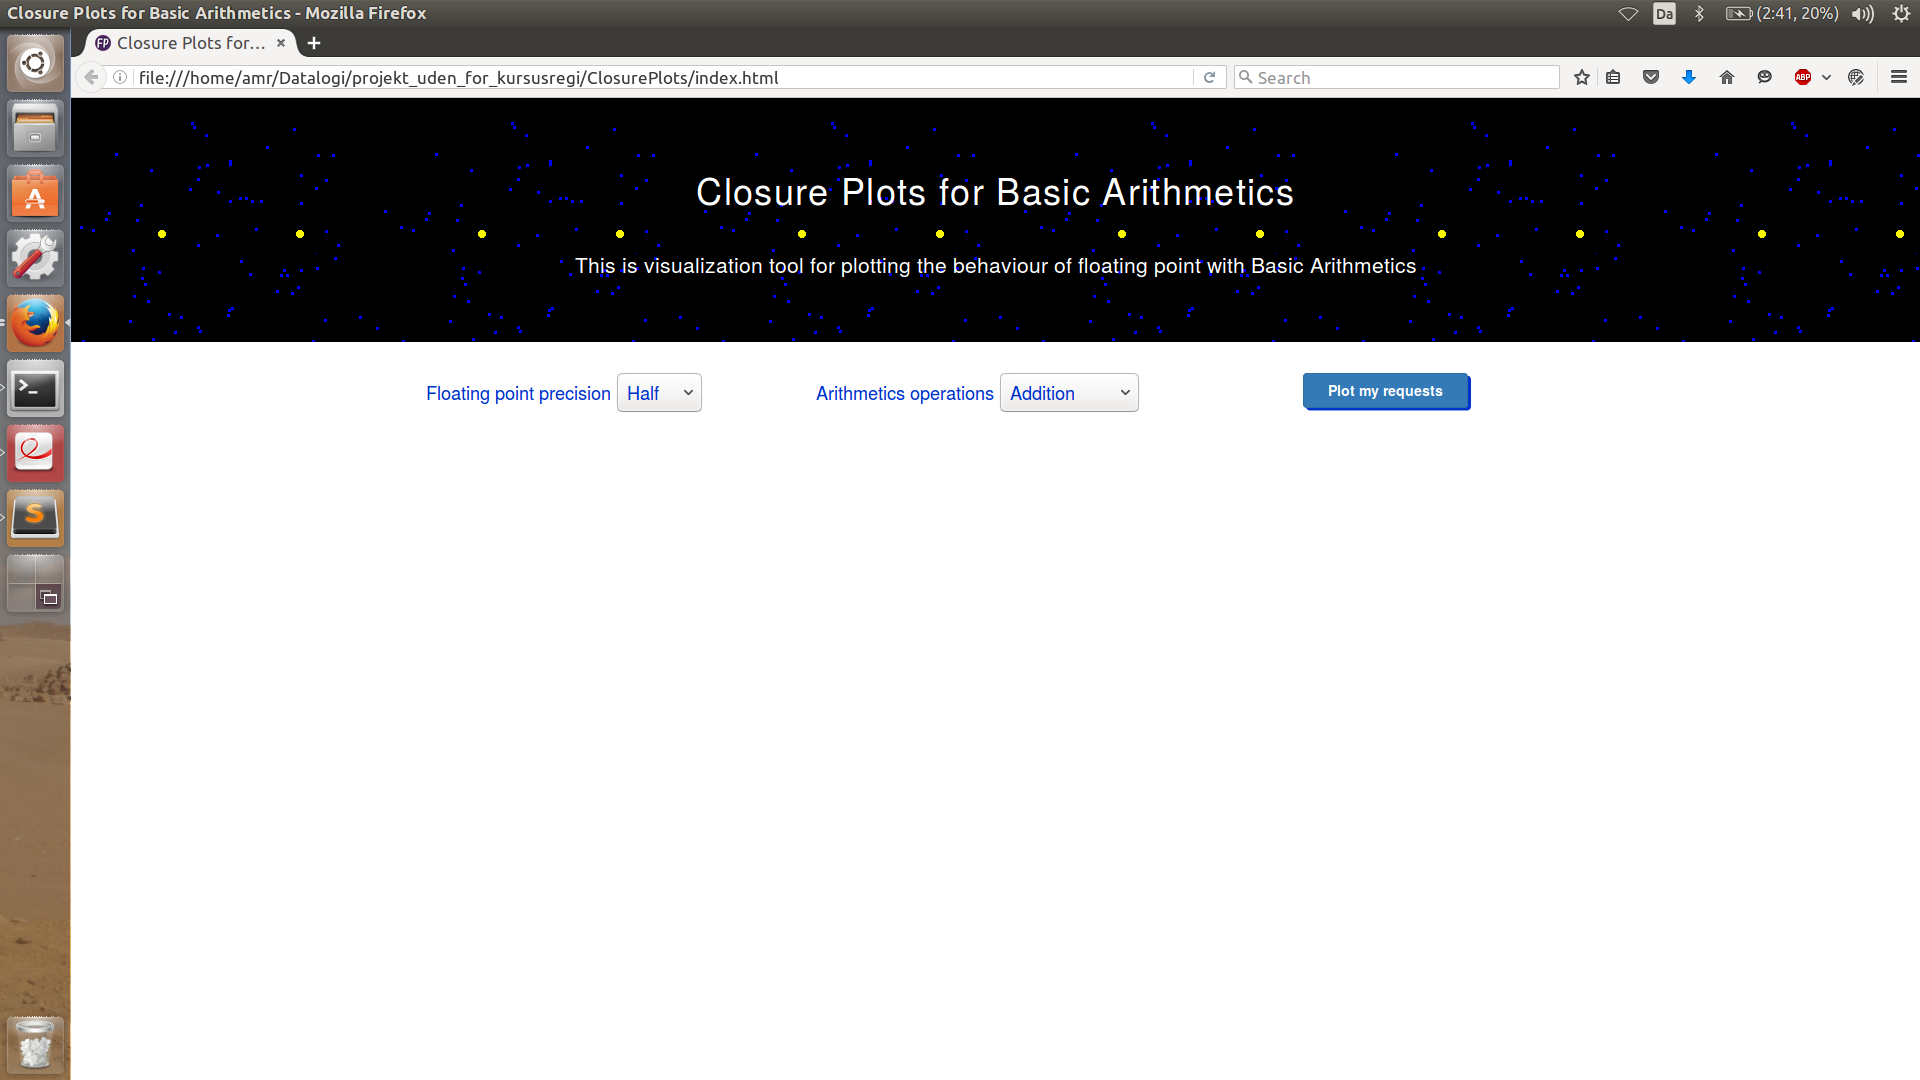
\includegraphics[width=0.55\textwidth]{offline}
    \caption{offline-mode}
    \label{offline}
\end{figure}
\begin{figure}[h]
    \centering
    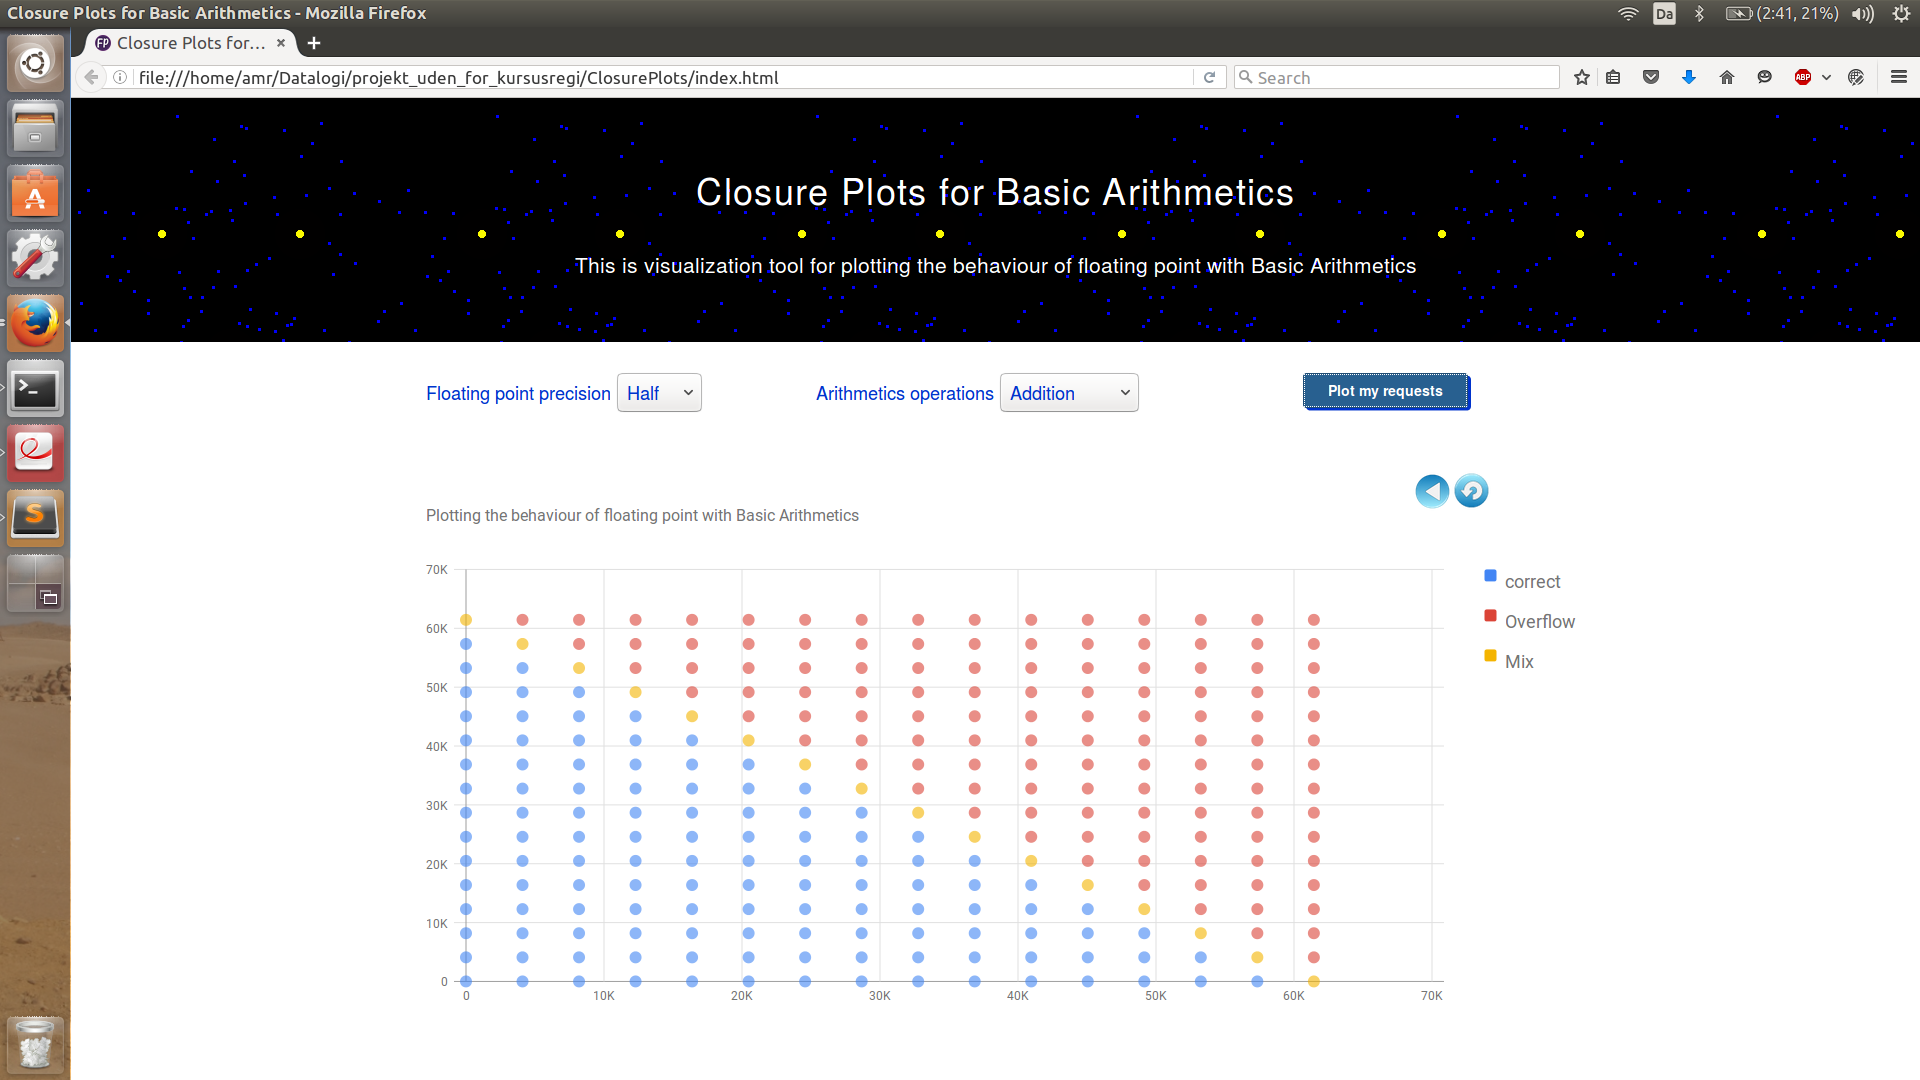
\includegraphics[width=0.55\textwidth]{half-add}
    \caption{addition operation with bit-width Half}
    \label{half-add}
\end{figure}
\begin{figure}[h]
    \centering
    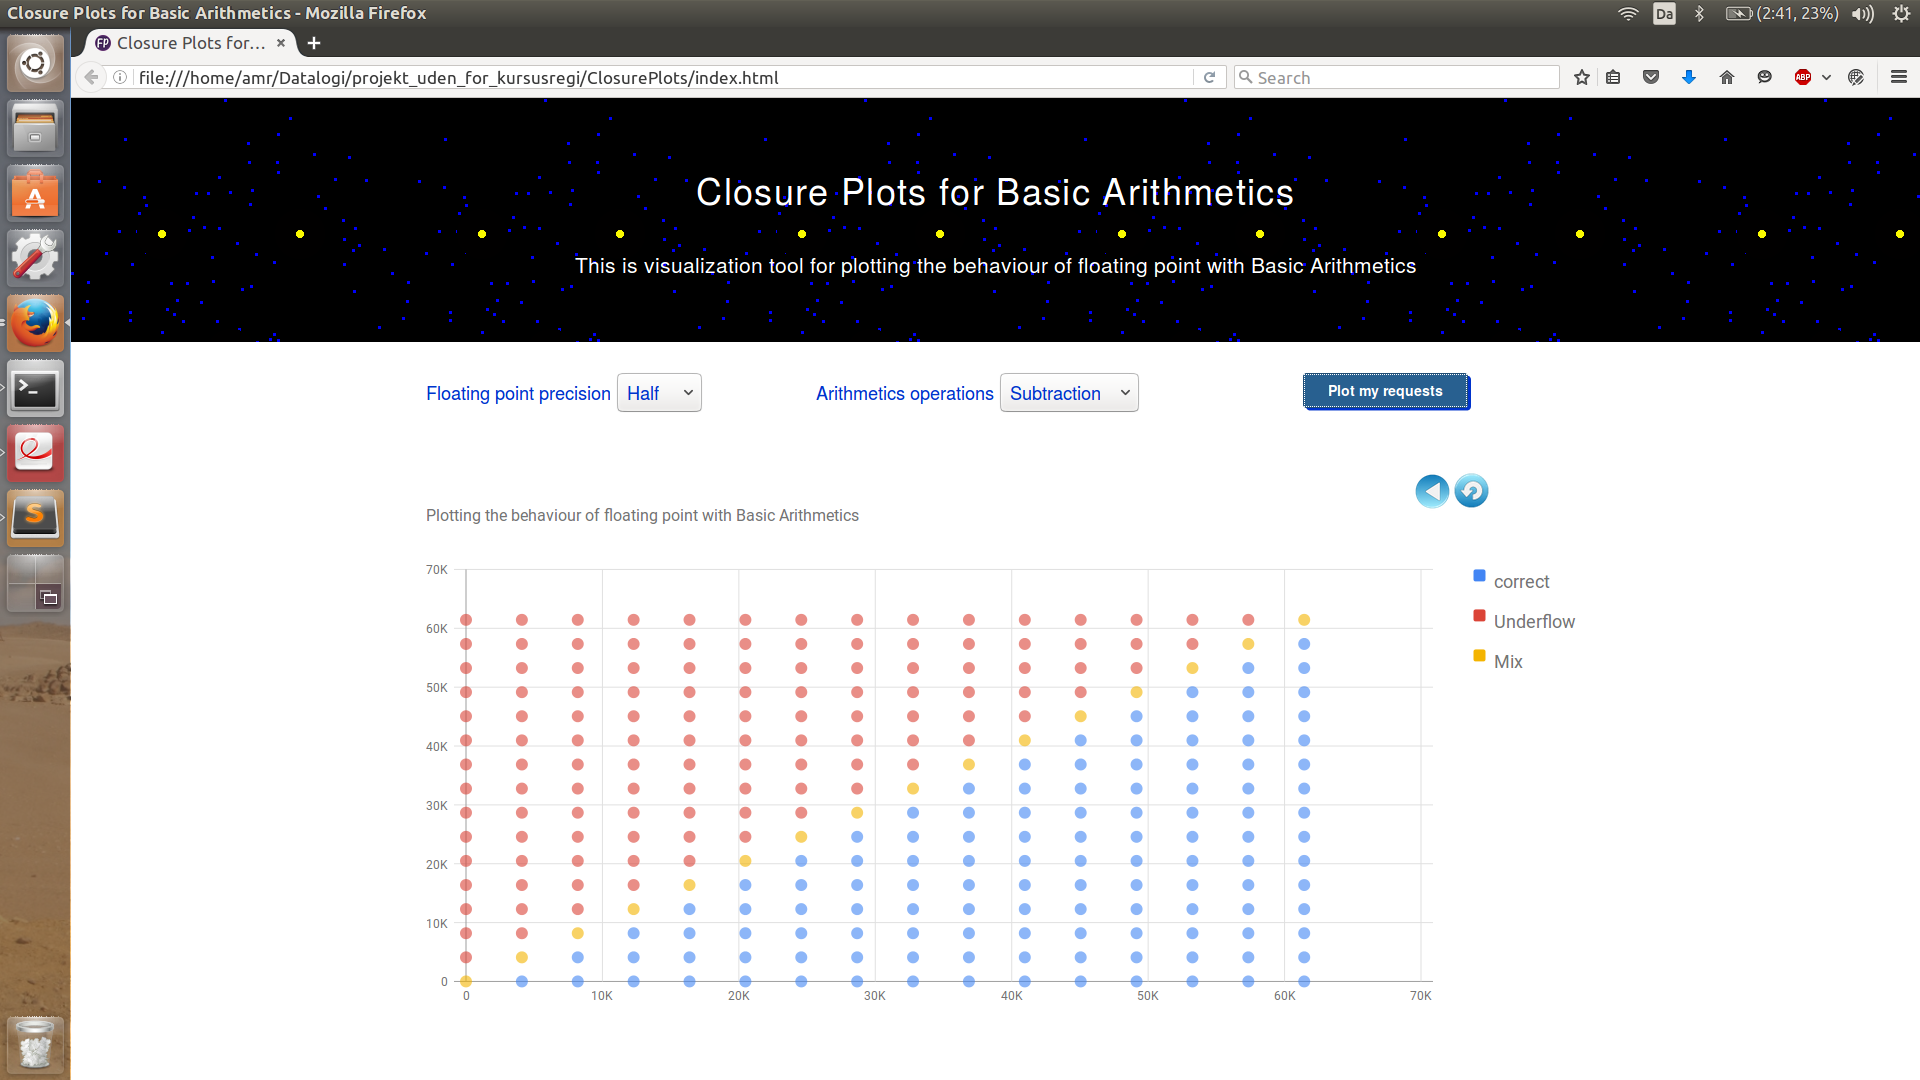
\includegraphics[width=0.55\textwidth]{half-sub}
    \caption{Subtraction operation with bit-width Half}
    \label{half-sub}
\end{figure}
\begin{figure}[h]
    \centering
    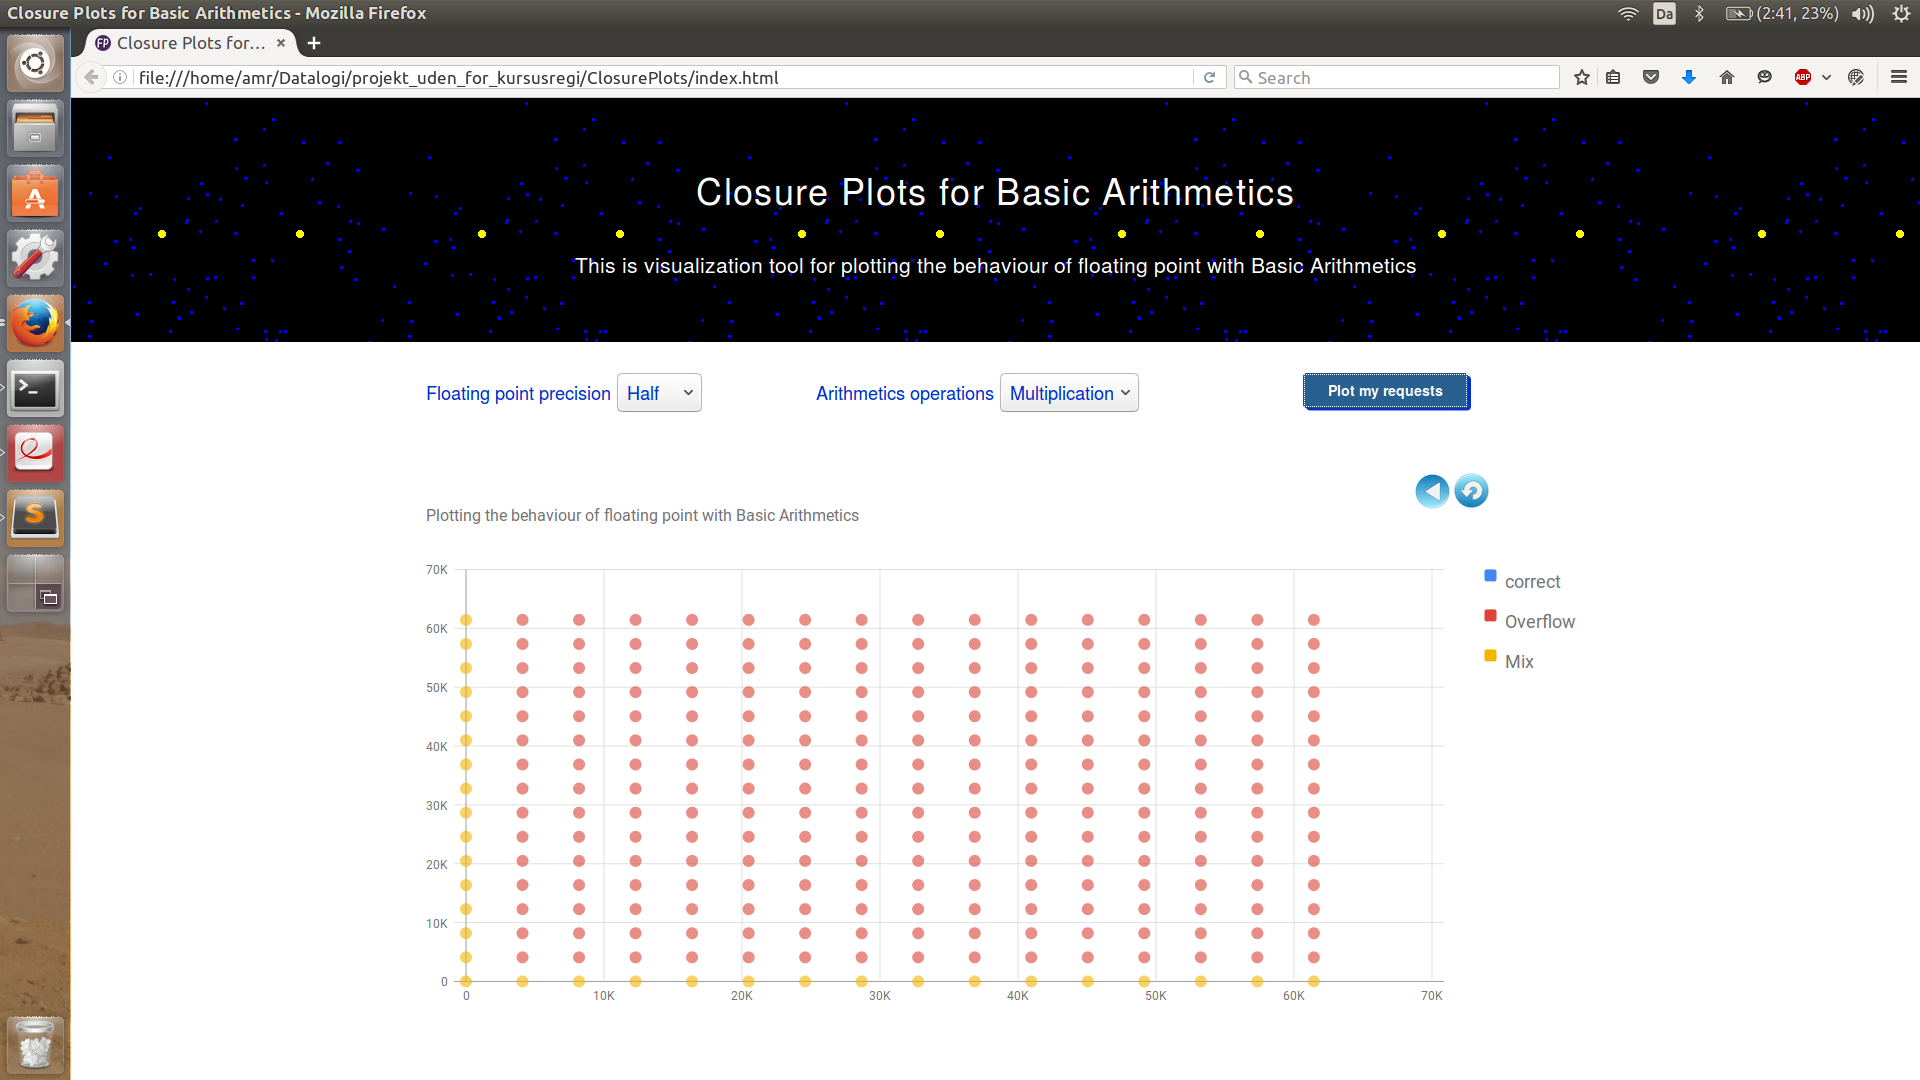
\includegraphics[width=0.55\textwidth]{half-mult}
    \caption{Multiplication operation with bit-width Half}
    \label{half-mult}
\end{figure}
\begin{figure}[h]
    \centering
    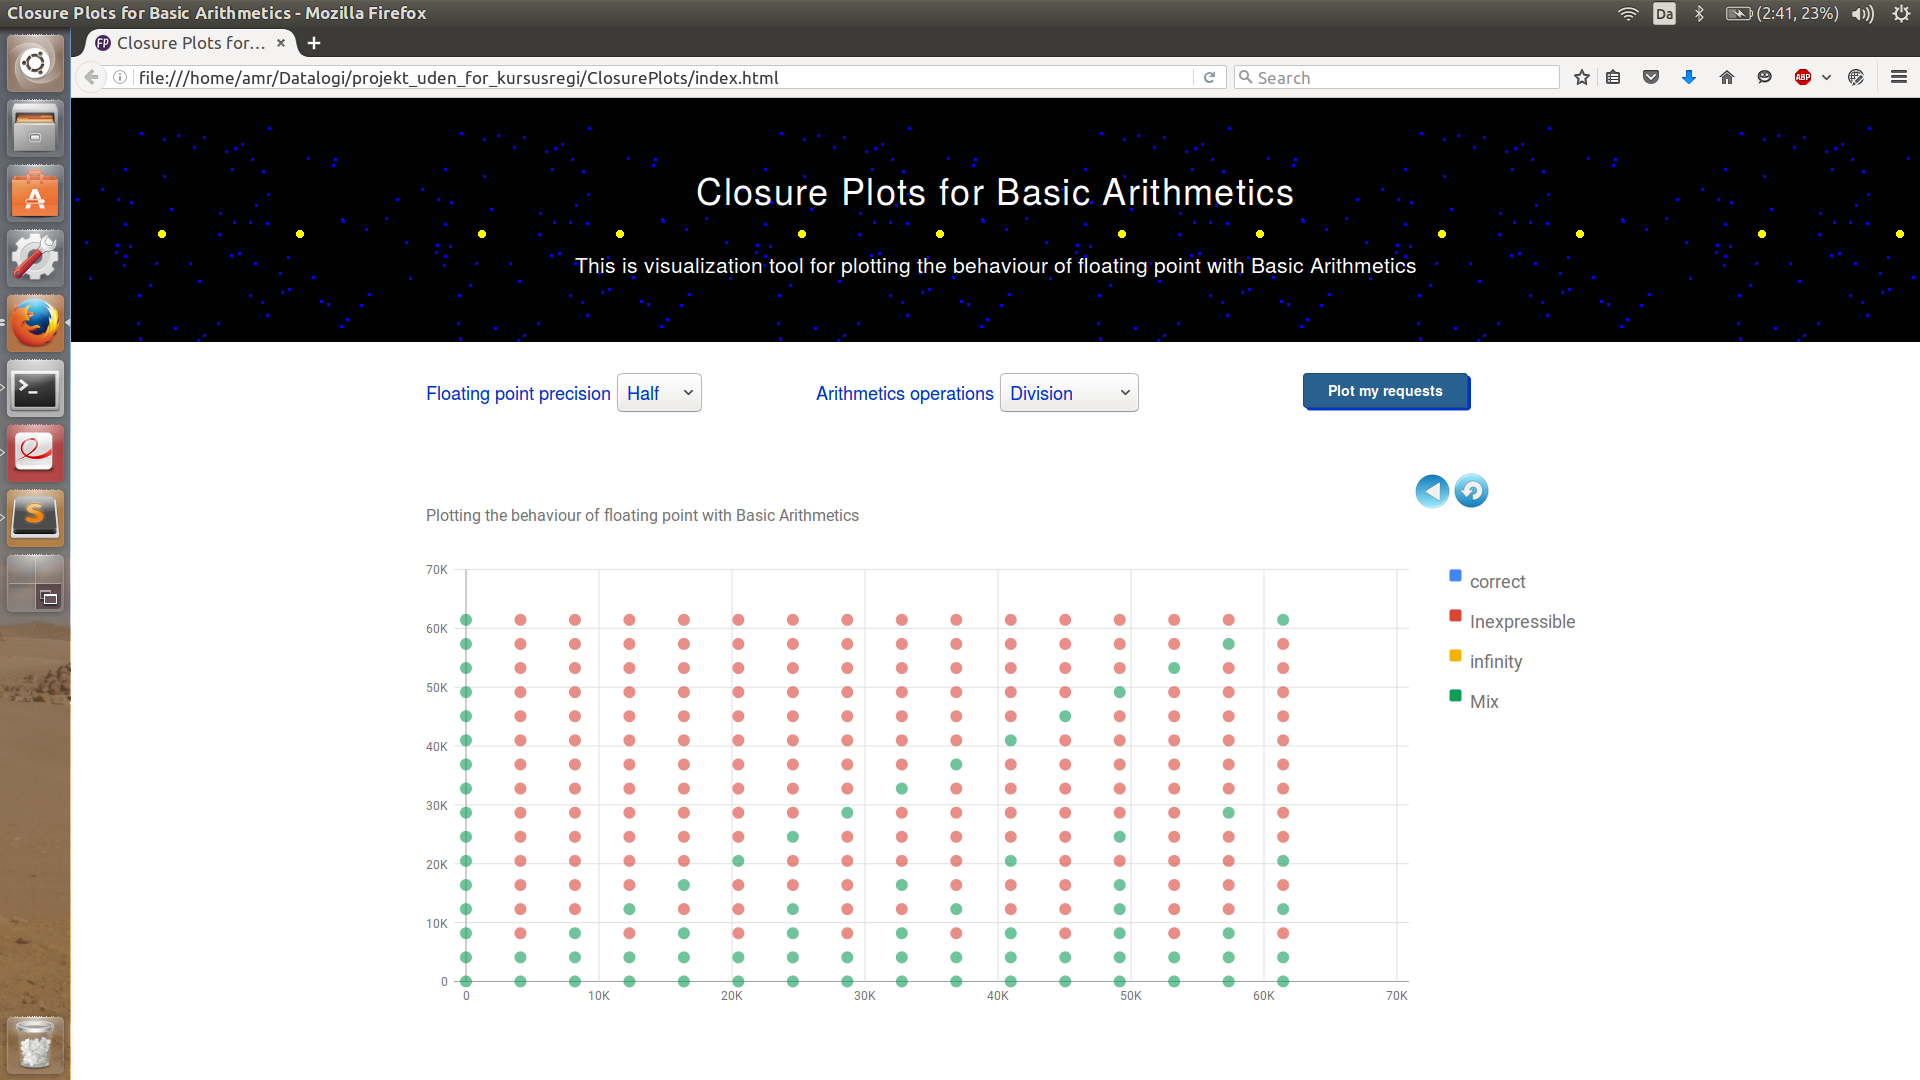
\includegraphics[width=0.55\textwidth]{half-div}
    \caption{Division operation with bit-width Half}
    \label{half-div}
\end{figure}
%%%%%%%%%%%%%%%%%%%%%%%%
\begin{figure}[h]
    \centering
    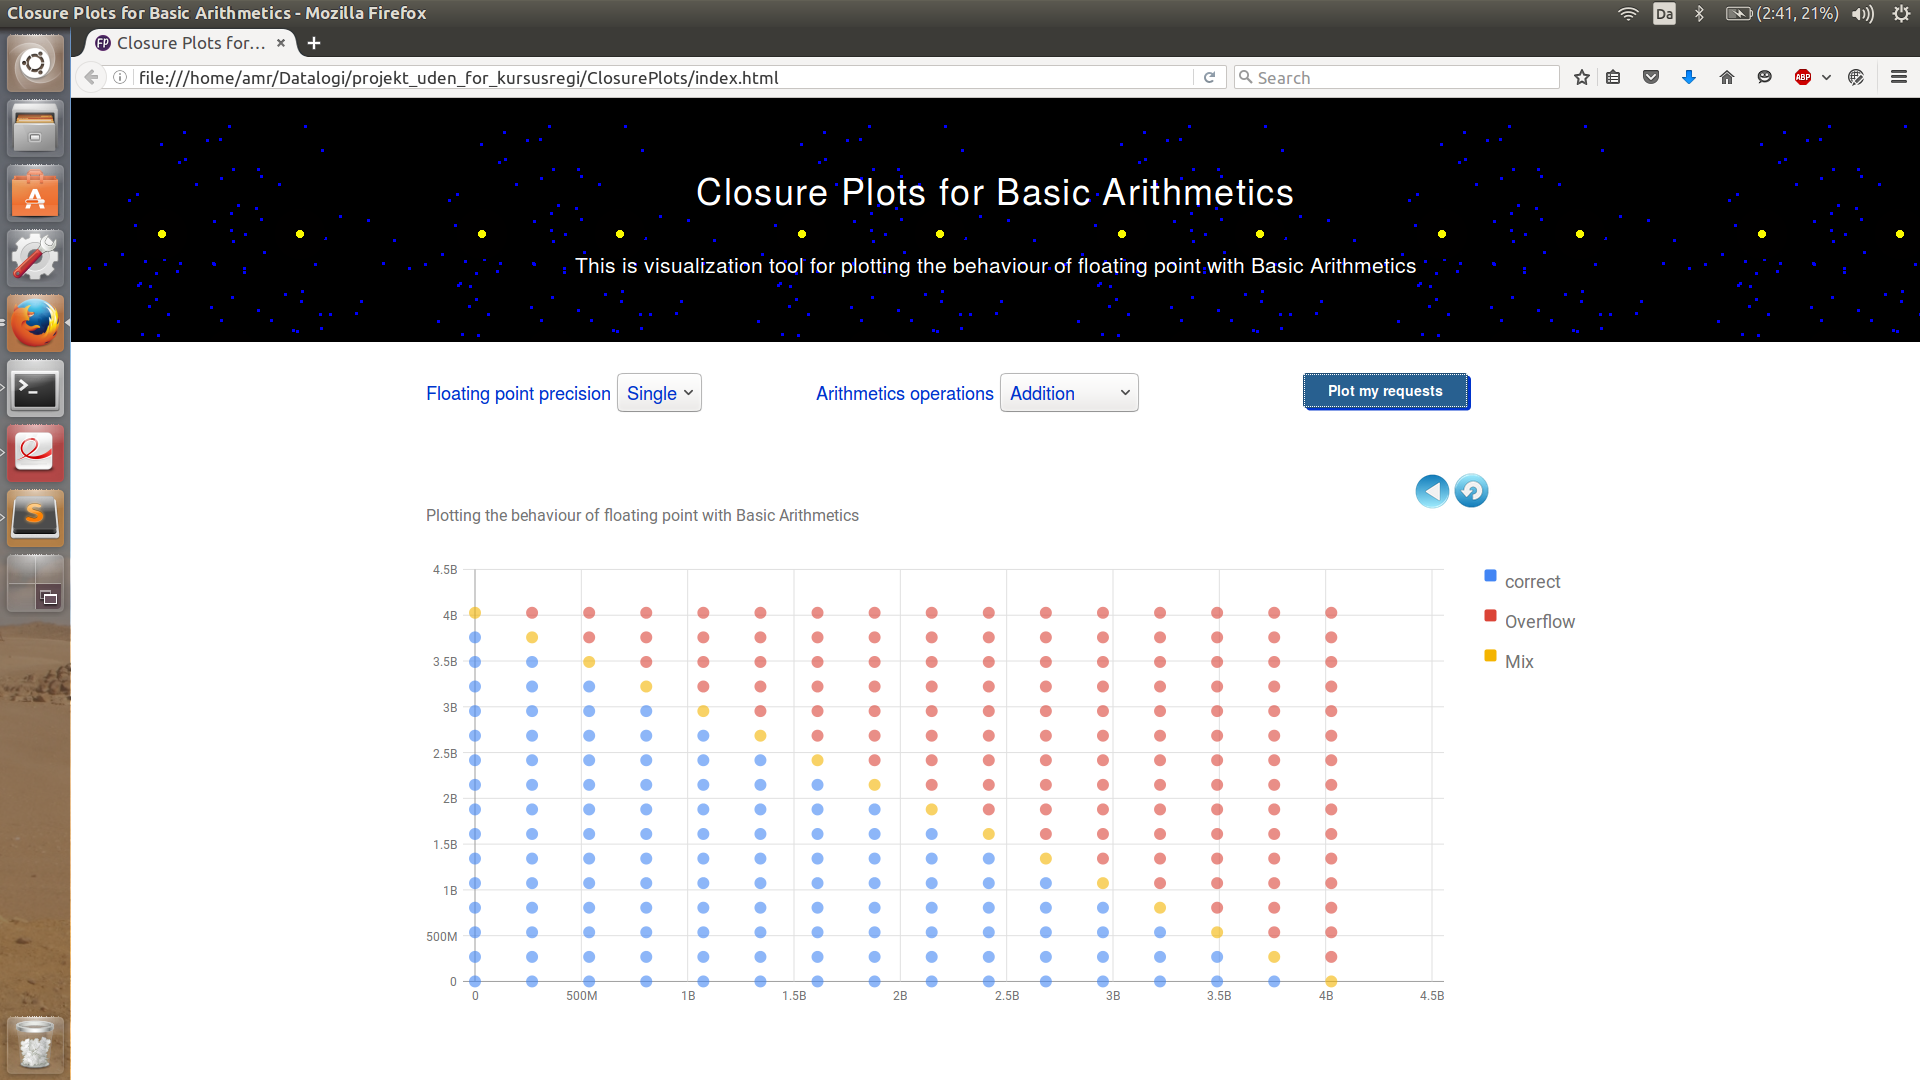
\includegraphics[width=0.55\textwidth]{single-add}
    \caption{addition operation with bit-width single}
    \label{single-add}
\end{figure}
\begin{figure}[h]
    \centering
    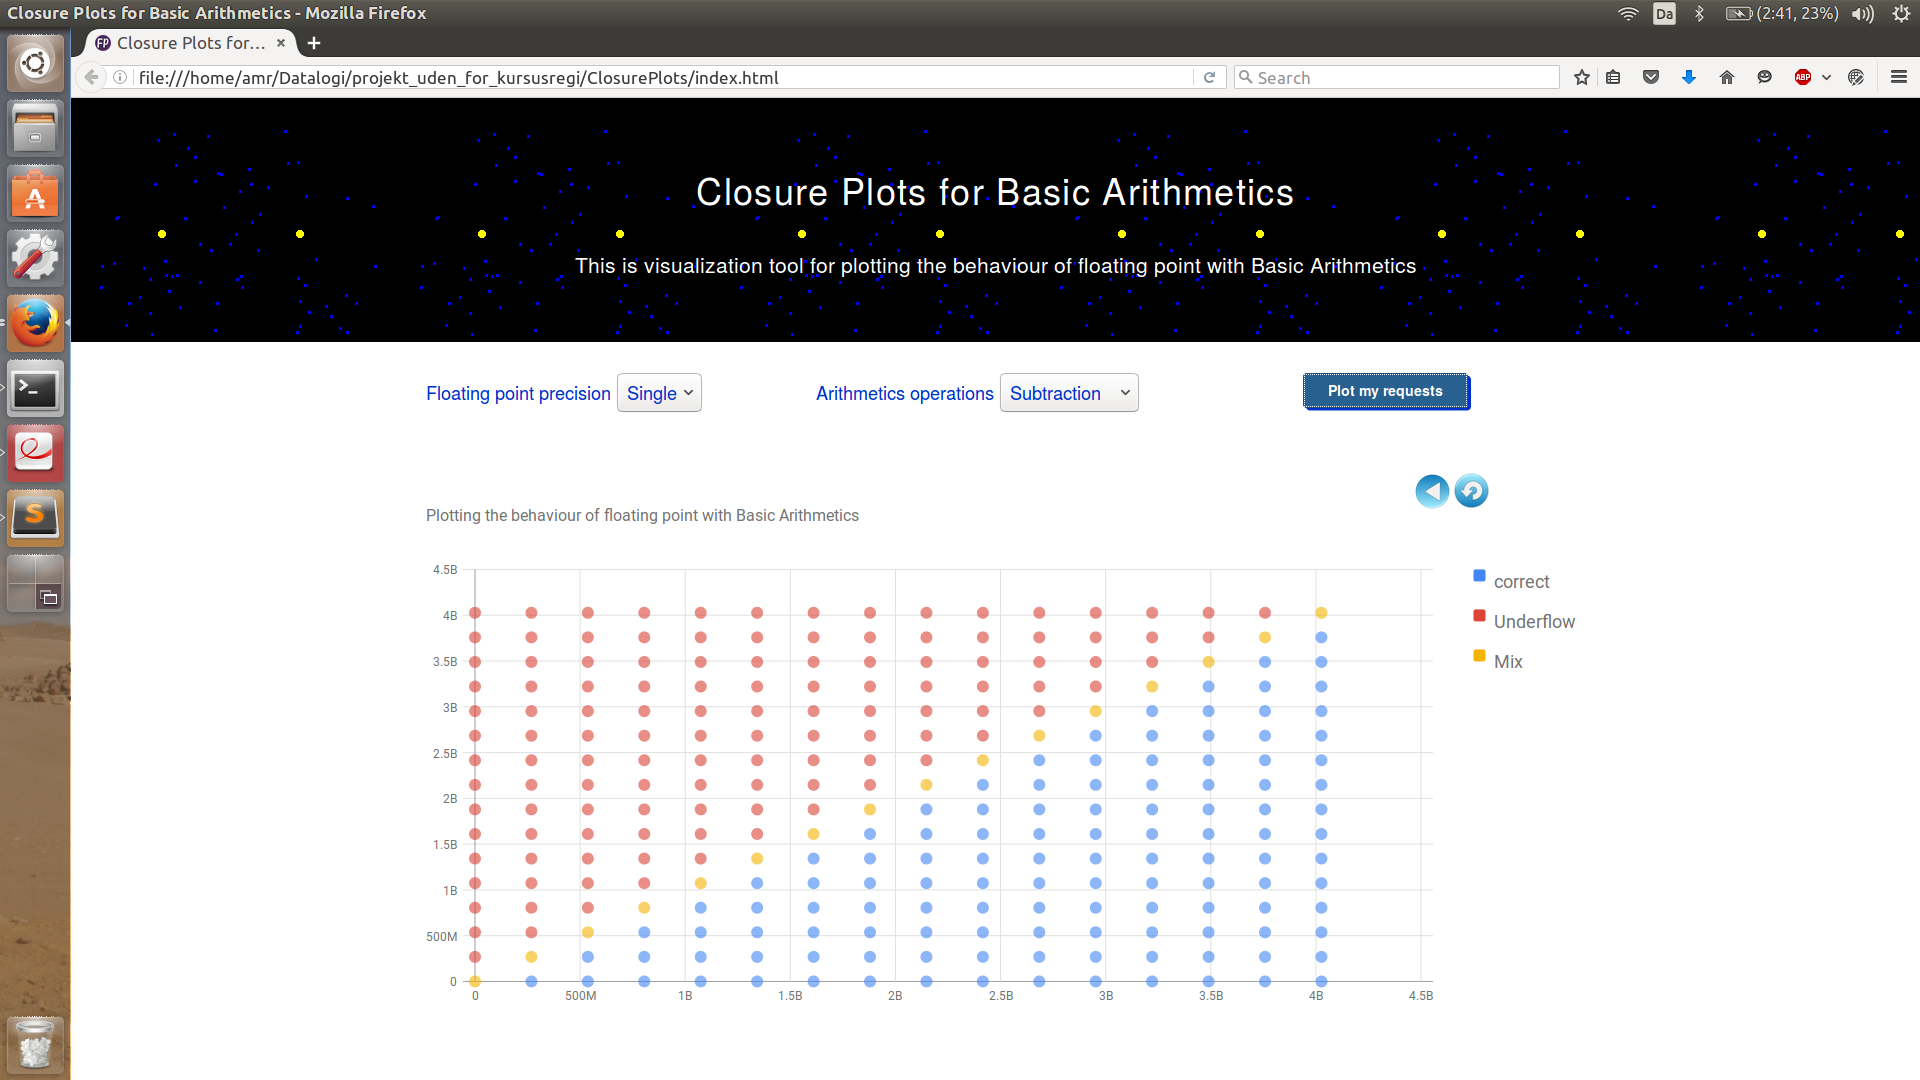
\includegraphics[width=0.55\textwidth]{single-sub}
    \caption{Subtraction operation with bit-width single}
    \label{single-sub}
\end{figure}
\begin{figure}[h]
    \centering
    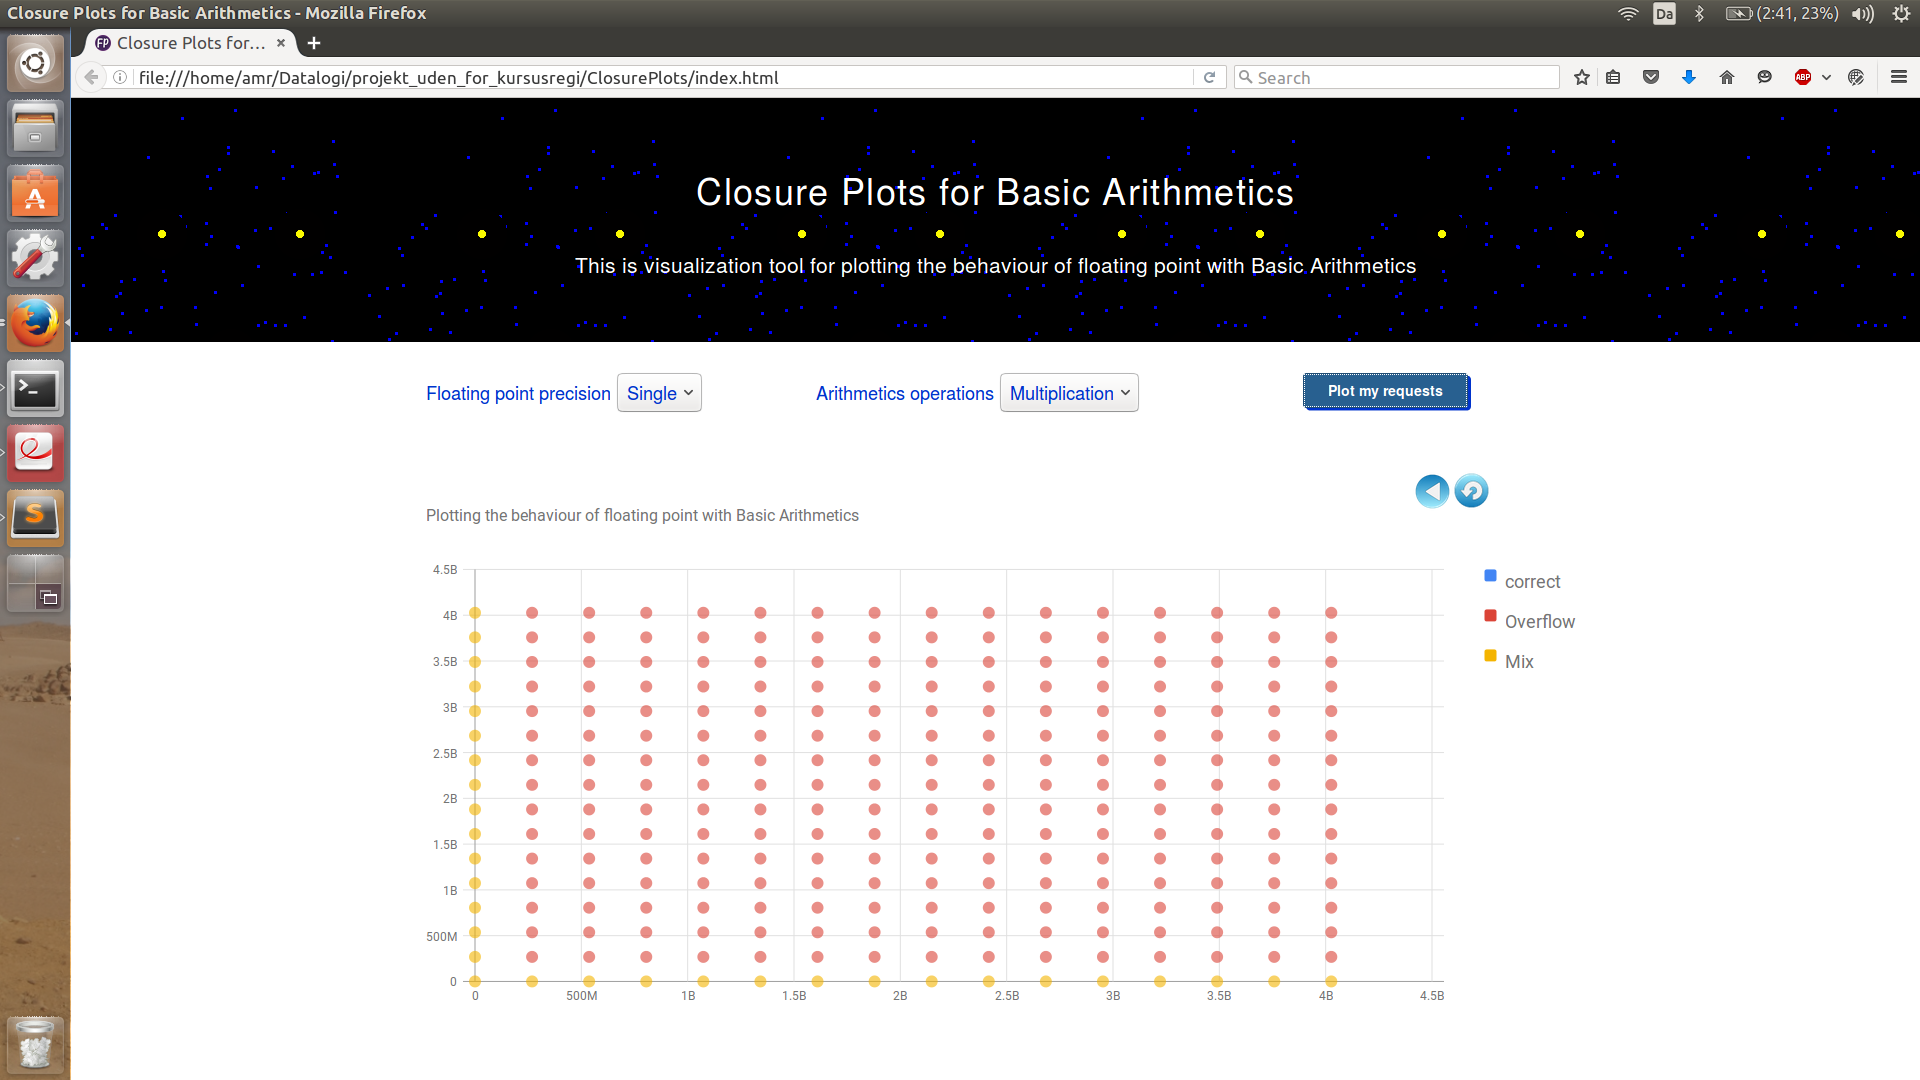
\includegraphics[width=0.55\textwidth]{single-mult}
    \caption{Multiplication operation with bit-width single}
    \label{single-mult}
\end{figure}
\begin{figure}[h]
    \centering
    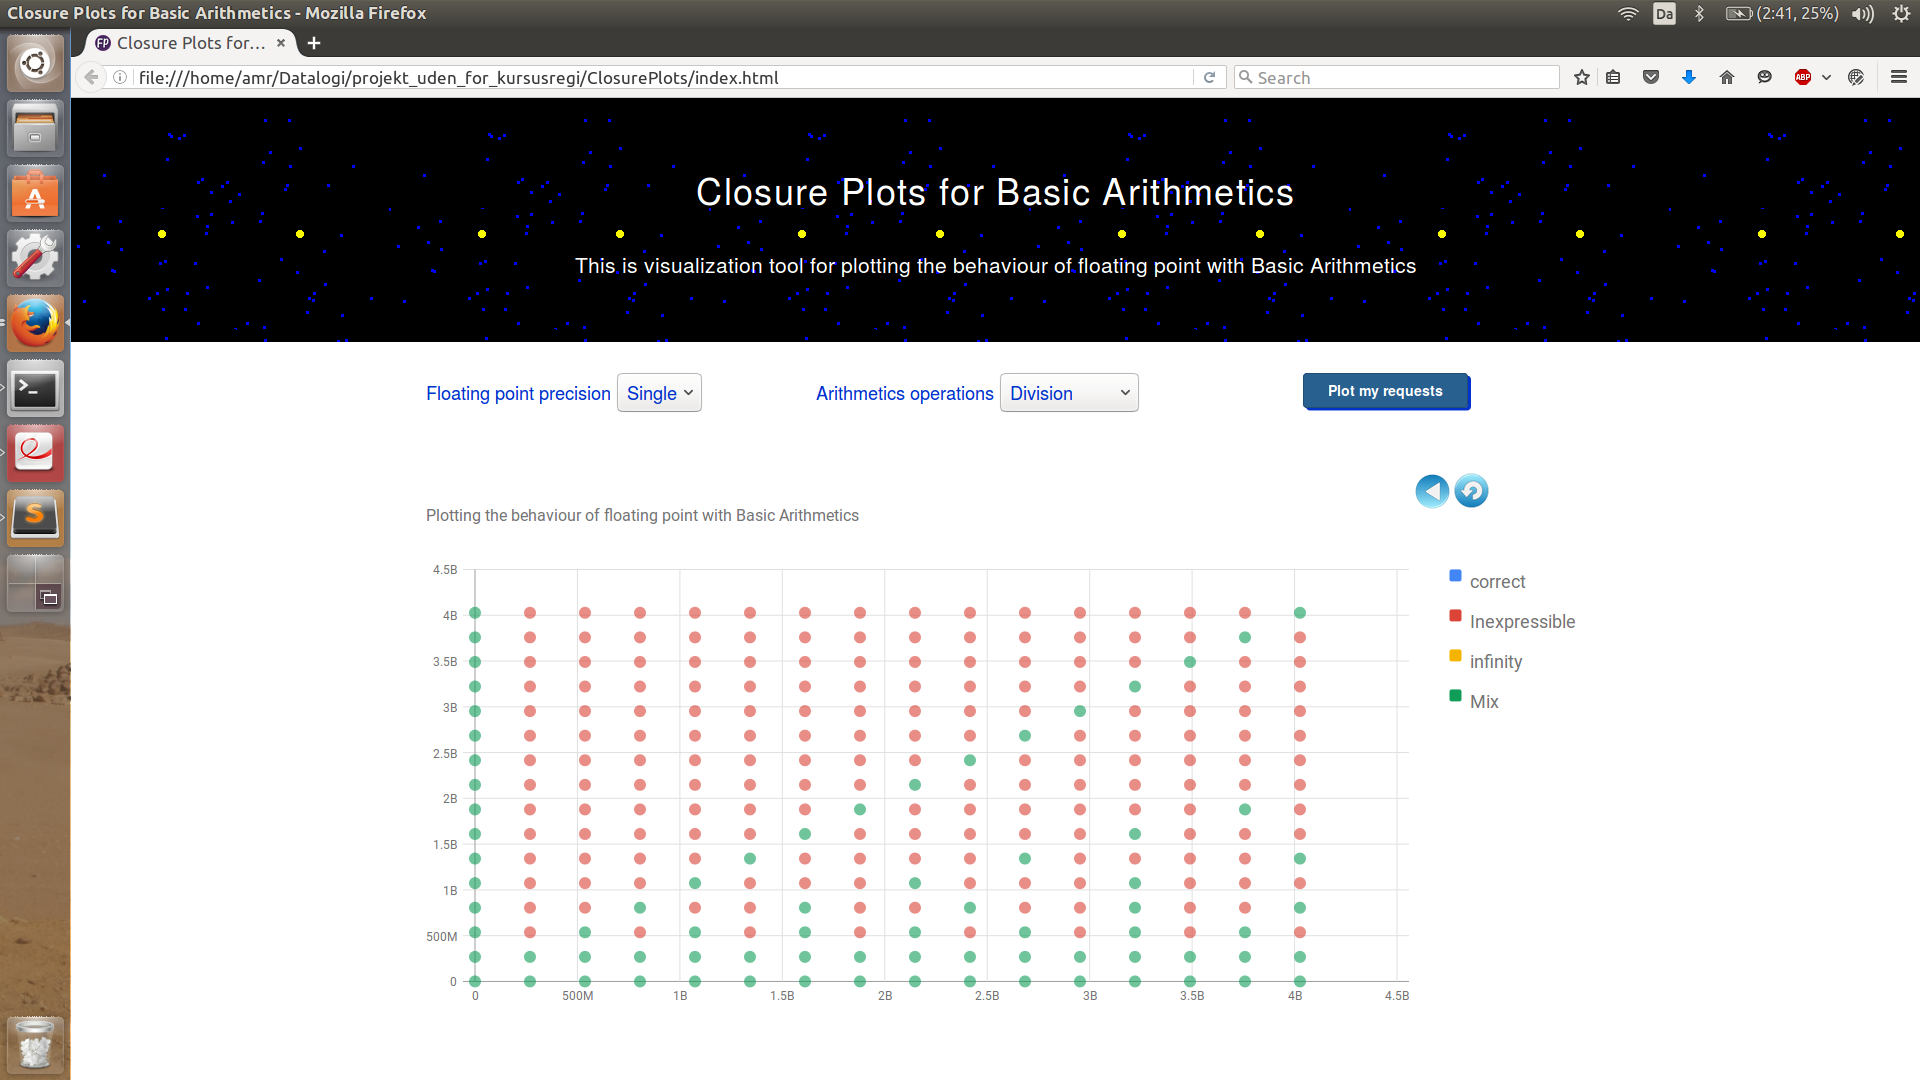
\includegraphics[width=0.55\textwidth]{single-divi}
    \caption{Division operation with bit-width single}
    \label{single-div}
\end{figure}
\begin{figure}[h]
    \centering
    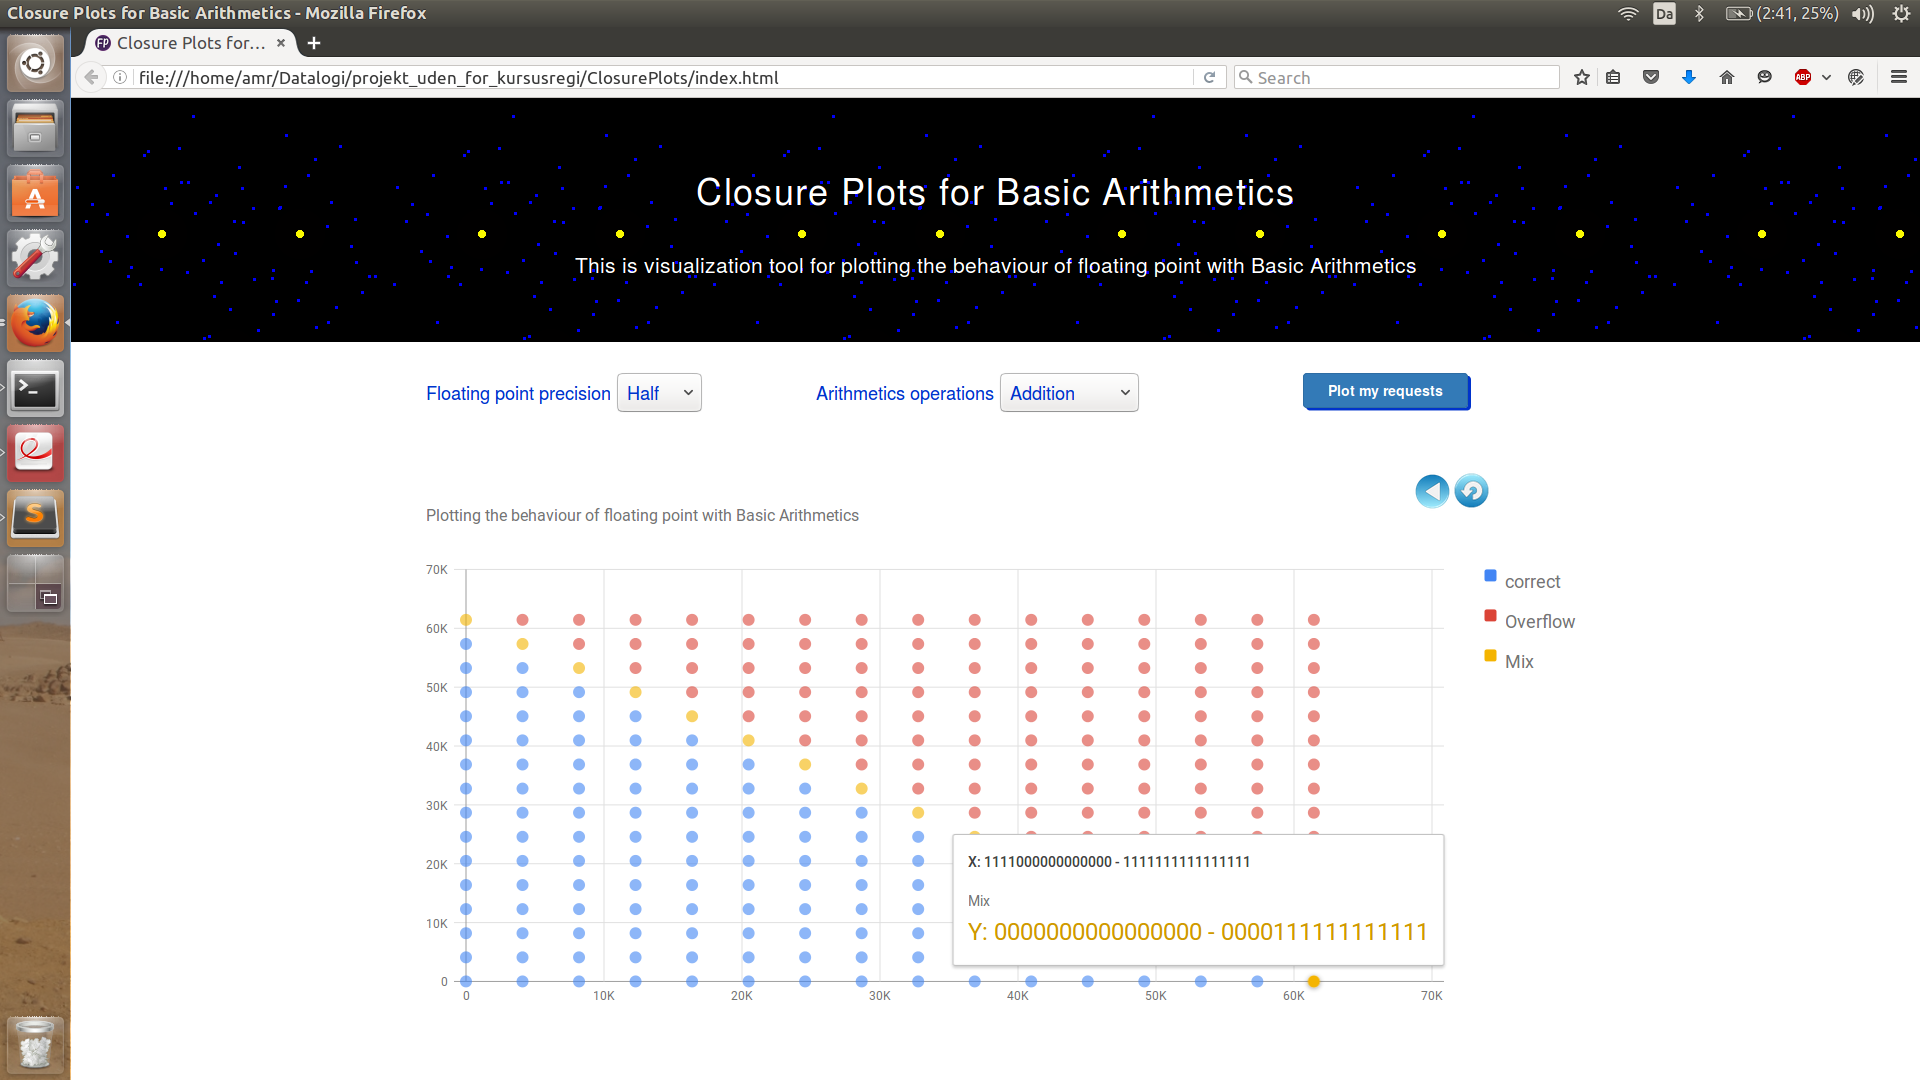
\includegraphics[width=0.55\textwidth]{first-stage-half-add}
    \caption{The first stage at the chart with bit-width Half to the addition operation}
    \label{first-stage}
\end{figure}
\begin{figure}[h]
    \centering
    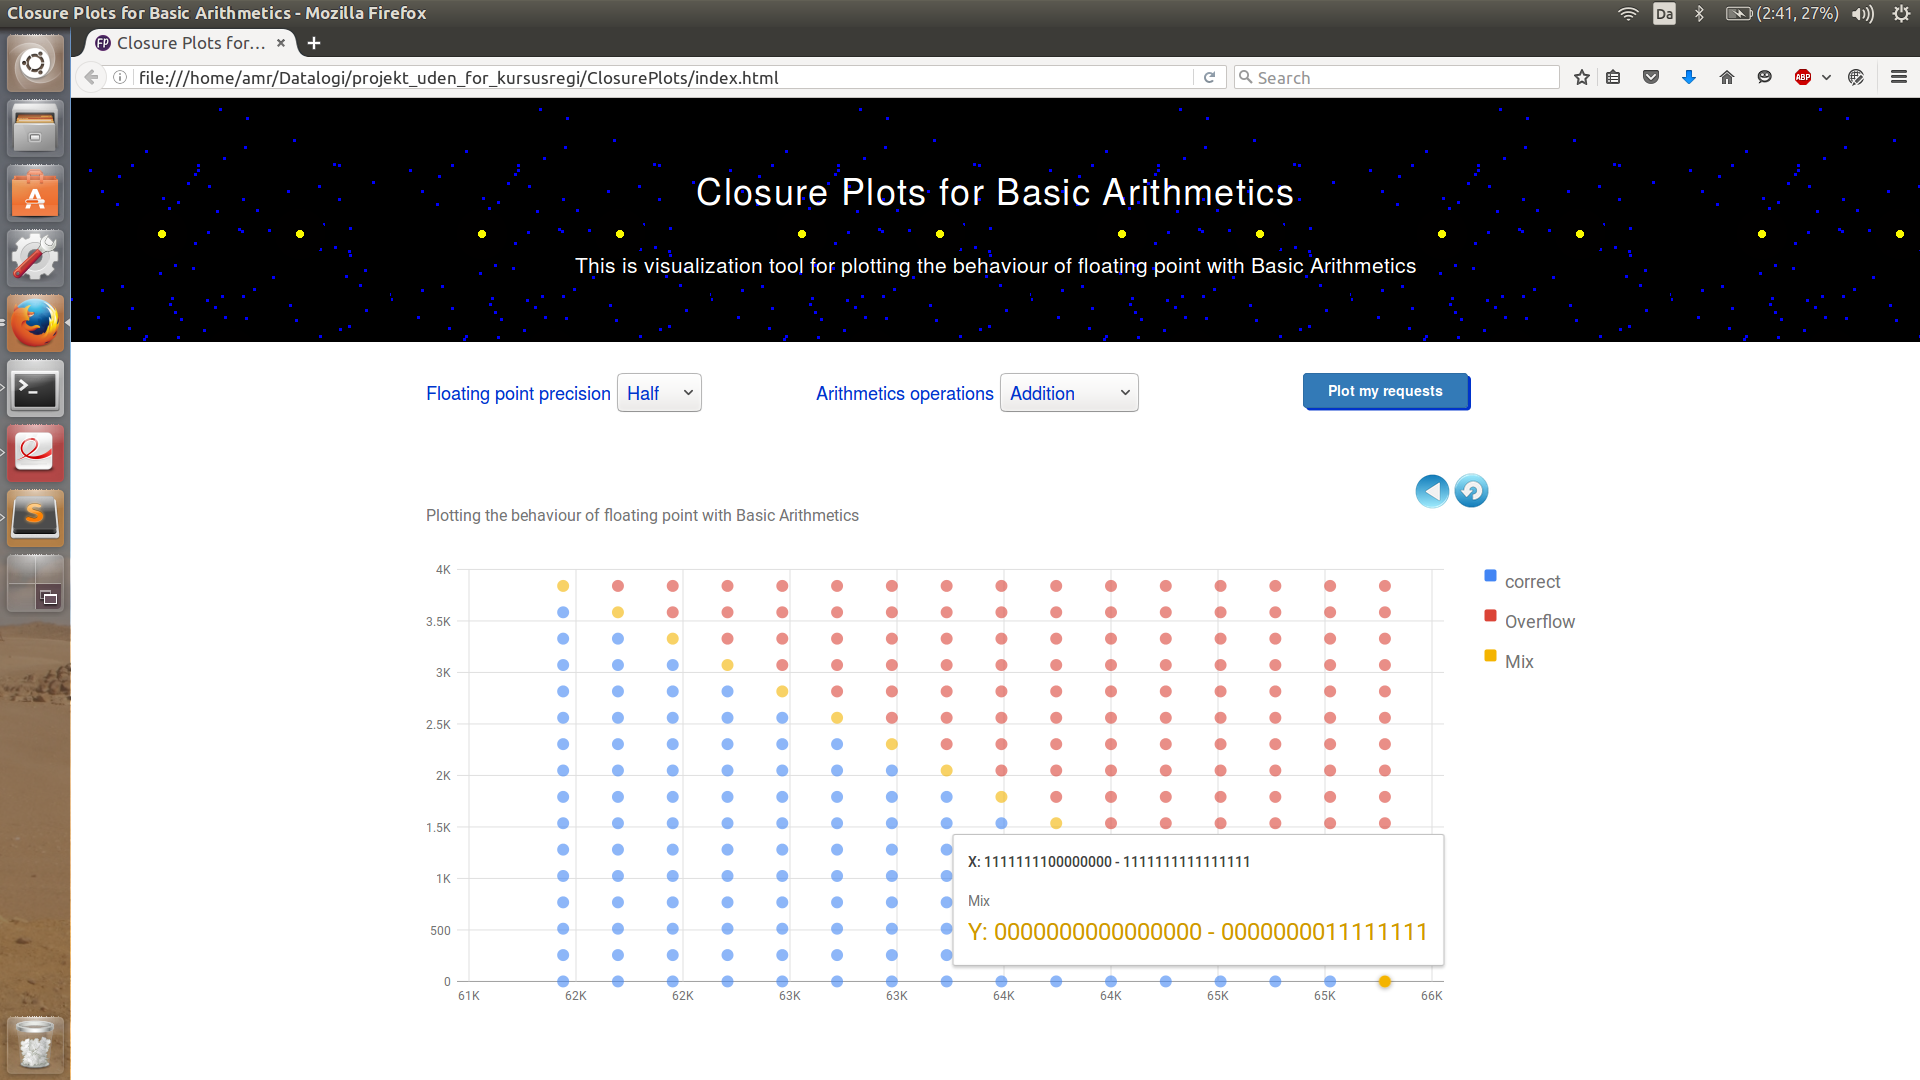
\includegraphics[width=0.55\textwidth]{second-stage-half-add}
    \caption{The second stage at the chart with bit-width Half to the addition operation}
    \label{second-stage}
\end{figure}
\begin{figure}[h]
    \centering
    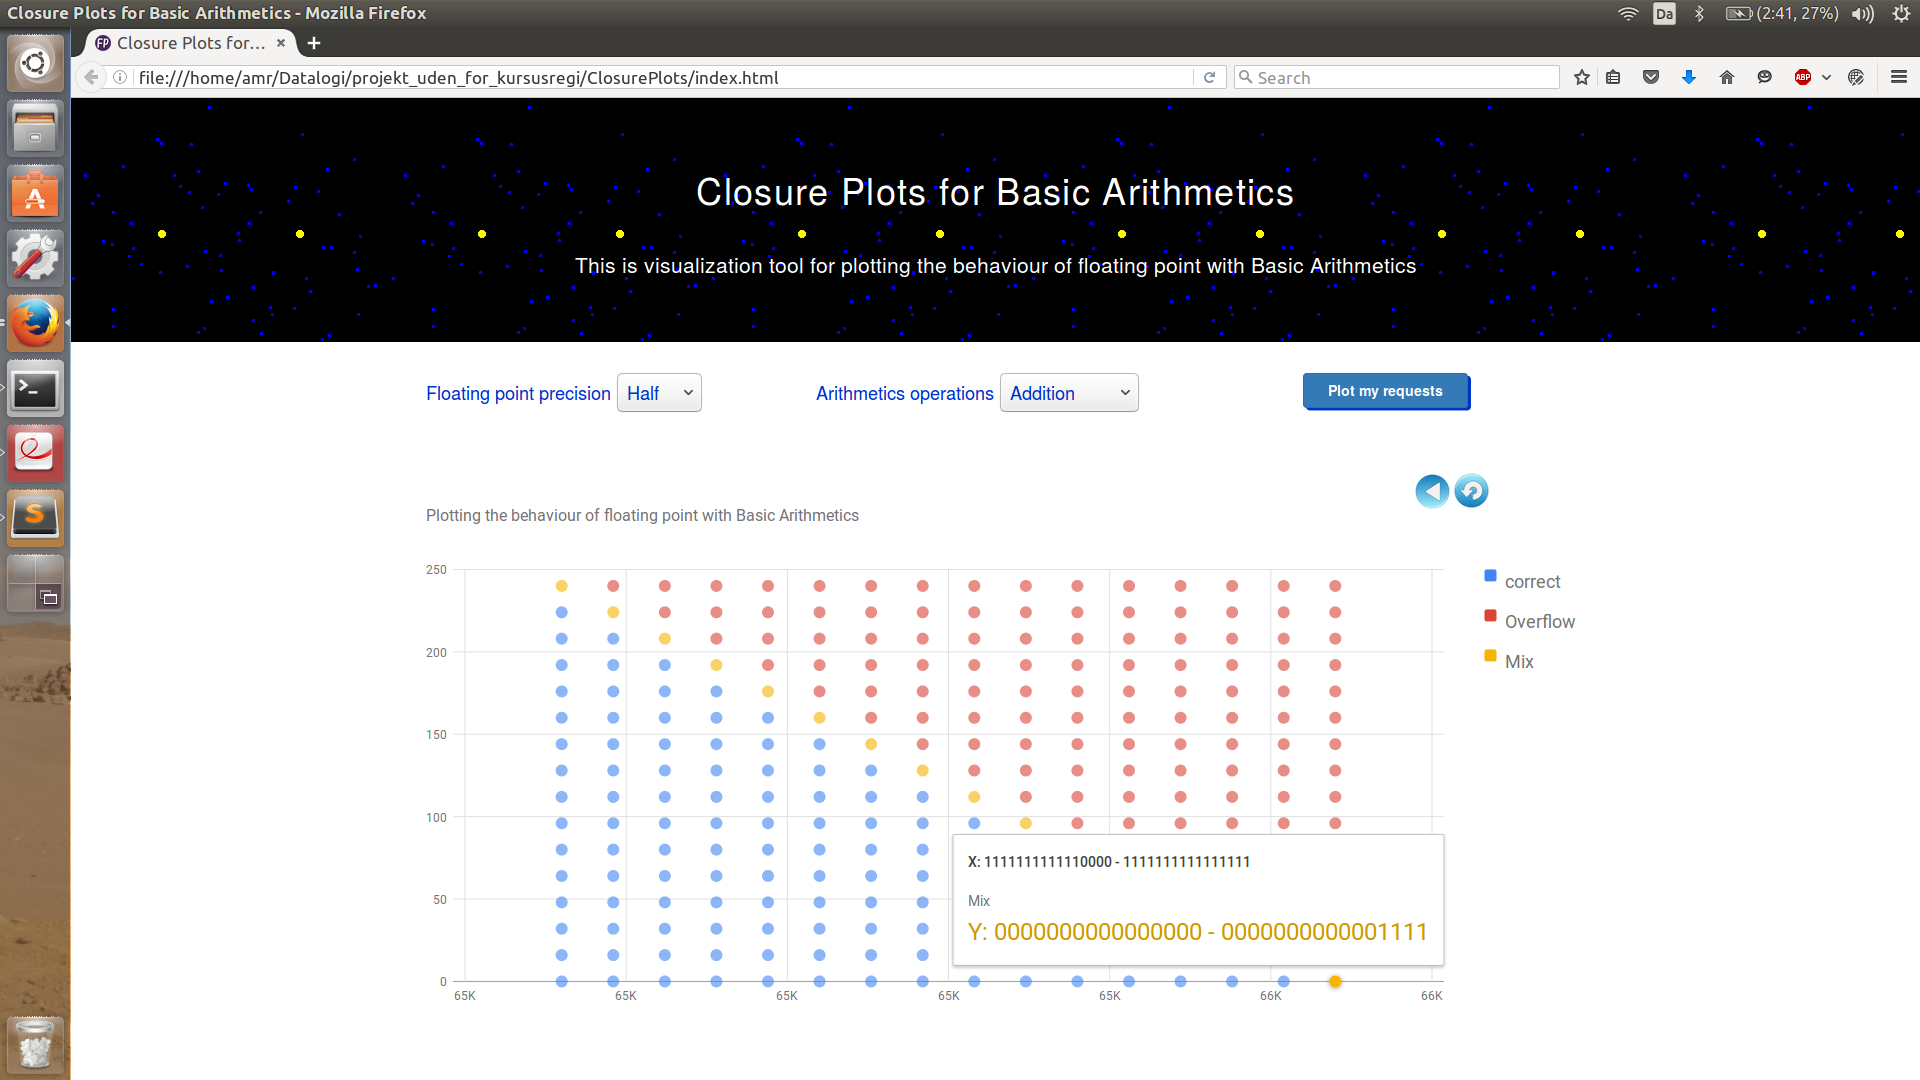
\includegraphics[width=0.55\textwidth]{third-stage-half-add}
    \caption{The third stage at the chart with bit-width Half to the addition operation }
    \label{third-stage}
\end{figure}
\begin{figure}[h]
    \centering
    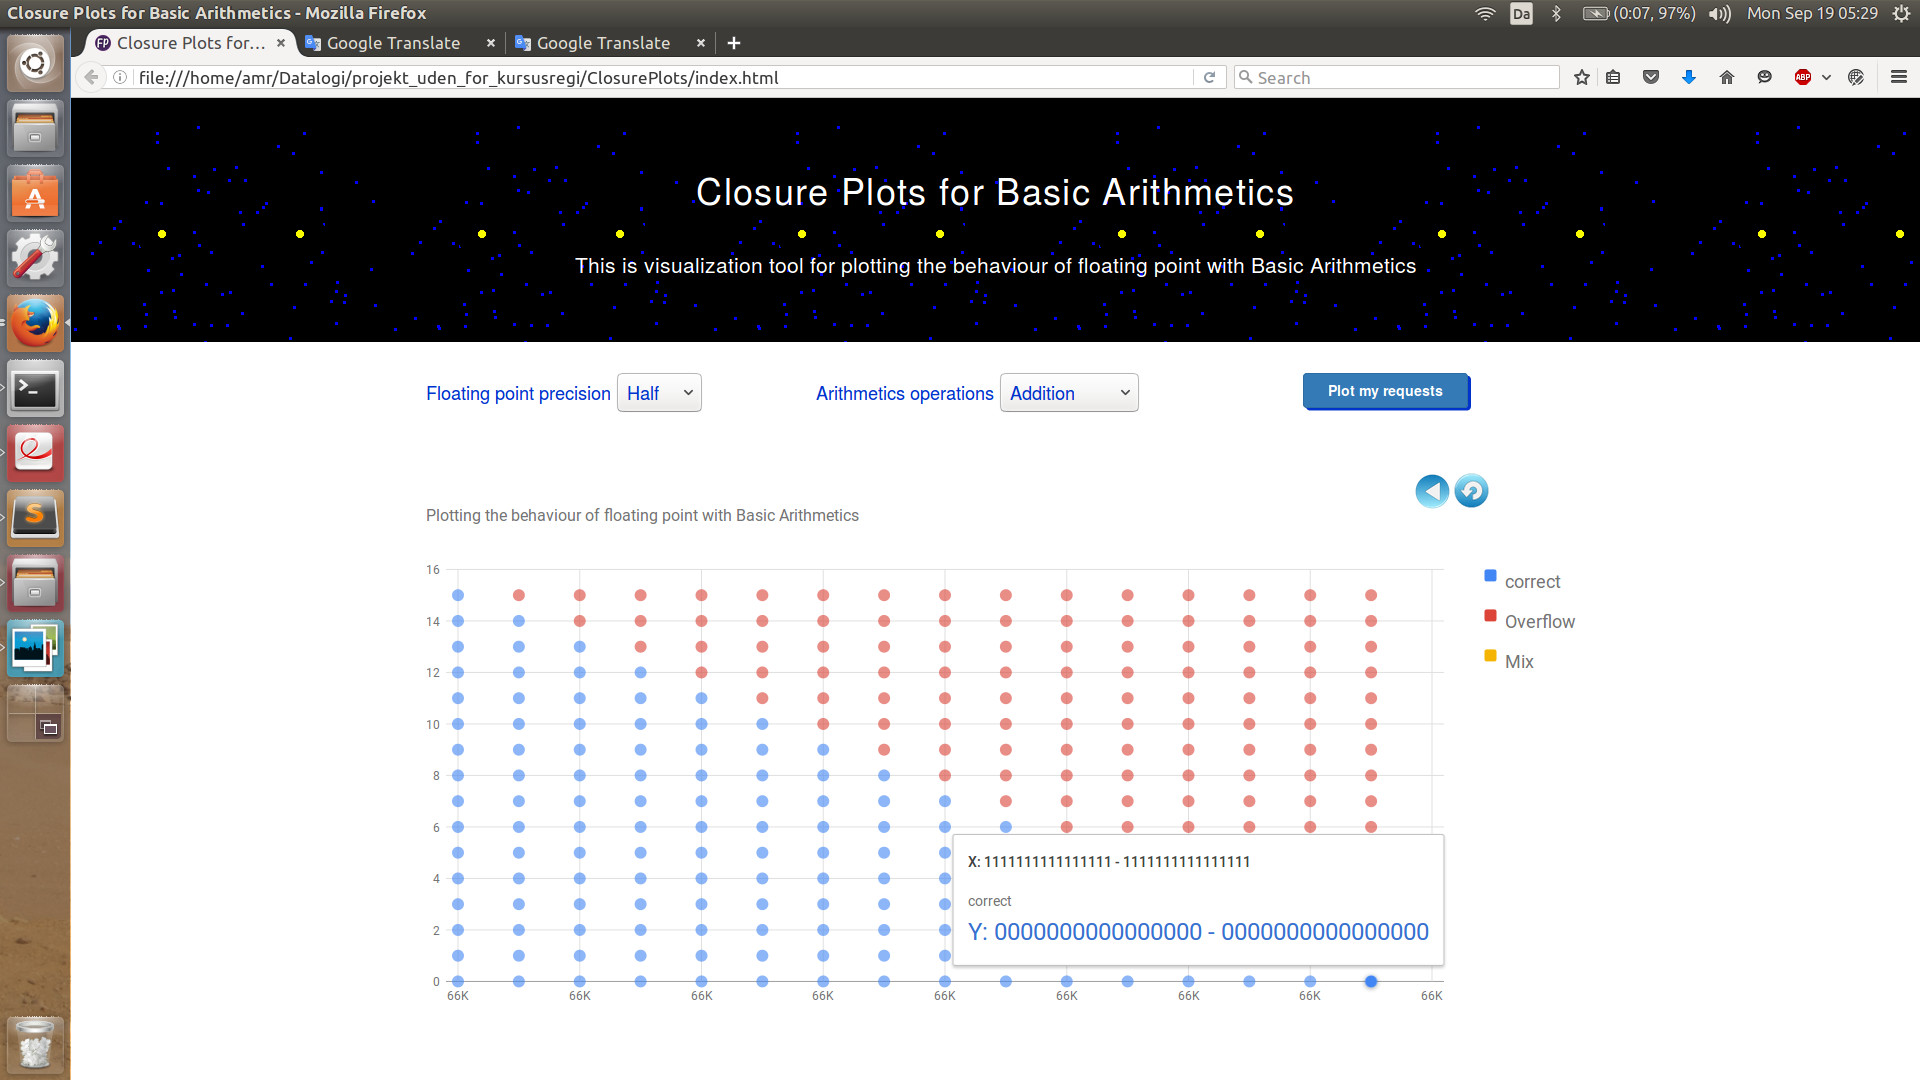
\includegraphics[width=0.55\textwidth]{last-stage-half-add}
    \caption{The last stage at the chart with bit-width Half to the addition operation }
    \label{last-stage}
\end{figure}
\end{document}
